\documentclass[12pt,a4j,dvipdfmx]{jarticle}
%---------------------------------------------------
\usepackage{hyperref}
\usepackage{pxjahyper}
\usepackage{bm}
\usepackage{graphicx}
\usepackage{amssymb,amsmath}
\usepackage{ascmac}
\usepackage{float}
\usepackage{setspace}
\usepackage[dvips,usenames]{color}
\usepackage{colortbl}
\usepackage{algorithm}
\usepackage{algorithmic}
\usepackage{setspace}
\usepackage{subfigure}
%---------------------------------------------------
\definecolor{bl}{rgb}{0.94,0.97,1}
\definecolor{gr}{rgb}{0.5,0.5,0.5}
\makeatletter
\def\section{\newpage\@startsection {section}{1}{\z@}{2.3ex plus -1ex minus -.2ex}{2.3 ex plus .2ex}{\Large\bf}}
\makeatother
%---------------------------------------------------
\setlength{\textwidth}{160truemm}
\setlength{\textheight}{240truemm}
\setlength{\topmargin}{-14.5truemm}
\setlength{\oddsidemargin}{-0.5truemm}
\setlength{\headheight}{0truemm}
\setlength{\parindent}{1zw}
%---------------------------------------------------
\setstretch{1.2}
%---------------------------------------------------
\renewcommand{\subfigtopskip}{5pt}	% 図の上の隙間。上図の副題と下図の間。
\renewcommand{\subfigbottomskip}{0pt} % 図の下の隙間。副題と本題の間。
\renewcommand{\subfigcapskip}{-6pt}	% 図と副題の間
\renewcommand{\subcapsize}{\scriptsize} % 副題の文字の大きさ
%---------------------------------------------------
% ヘッダーとフッターの設定
\usepackage{fancyhdr}
\rhead{\leftmark}
\chead{}
\lhead{\rightmark}
\cfoot{\thepage}

\rfoot{}
\begin{document}
\thispagestyle{empty}
\begin{spacing}{1}
\begin{center}
\vspace*{3.5cm}
{\Huge トランジスタ回路の設計}\\
\vspace*{12.5cm}
{\Large 電気情報工学科4年後期}\\
{\Large 電気電子工学実験II}\\
\vspace*{1cm}

\end{center}

\newpage
\pagenumbering{roman}
\tableofcontents
\end{spacing}
\clearpage
\pagenumbering{arabic}
\pagestyle{fancy}
\setlength{\headheight}{5truemm}

\input{1_about_LTspice.tex}
\section{トランジスタ回路の設計}
トランジスタの基本的な増幅回路であるエミッタ接地増幅回路を設計する。
原理の説明とシミュレーション演習を並行して行うことで、電子回路の設計方法を習得する。

\subsection{2SC1815の直流増幅率測定}
\begin{description}
  \setlength{\parskip}{0cm} % 段落間
  \setlength{\itemsep}{0cm} % 項目間
  \item[ゴール] 専用測定器にトランジスタの足を差し込んで、増幅率を測定する。
  \item[キーワード] 直流増幅率
\end{description}
\section{トランジスタのDC特性(基本特性)について}
\begin{description}
  \setlength{\parskip}{0cm} % 段落間
  \setlength{\itemsep}{0cm} % 項目間
  \item[ゴール] $I_E$-$V_{BE}$ 特性、$I_C$-$I_B$ 特性、$I_C$-$V_{CE}$特性をLTspiceのシミュレーションで取得する。
  \item[キーワード] 直流電流増幅率、ダイオード特性
\end{description}
トランジスタは小さな信号を大きな信号に増幅できる特性を持つ半導体素子である。
3つの電極は、E(エミッタ) C(コレクタ) B(ベース) で構成される。今回は、NPNトランジスタを扱う。
\subsection{原理・計算}
NPNトランジスタ回路の原理図を下図に示す。
\begin{figure}[htbp]
  \begin{center}
  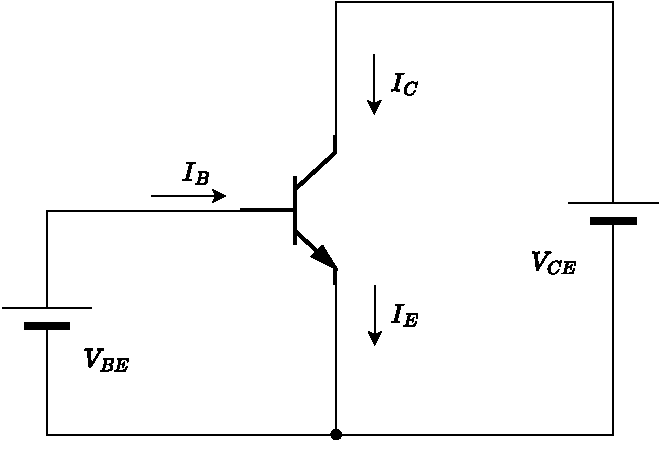
\includegraphics[width=0.5\linewidth]{img/24.pdf}
  \caption{NPNトランジスタ回路の原理図}
  \end{center}
\end{figure}
\\キルヒホッフの電流測より、
$$I_E = I_B+I_C$$
エミッタ接地直流増幅率を $\beta_0$ とすると、$$I_C = \beta_0I_B$$
また、ベース \- エミッタ間はpn接合ダイオードなので、エミッタ電流 $I_E$ は、
$$I_E \approx I_S\left[\exp\left(\frac{q}{kT}V_{BE}\right)-1\right]\approx I_S\exp\left(\frac{q}{kT}V_{BE}\right)$$
$I_S$はダイオードに逆方向の電圧がかかったときの微小な電流(1pA ～ 1nA)である。 $q$ は、電子の負荷、$k$ はボルツマン定数、
Tは絶対温度であり、$\frac{q}{kT}$ の値は、常温(300K)で約 38.7 V$^{-1}$ となる。
式を変形して、$$\ln I_E \approx \ln I_S + \frac{q}{kT}V_{BE}$$
$$\log I_E \approx \log I_S + \left(\frac{q}{kT}\log e\right)\cdot V_{BE}$$
となる。

\subsection{LTspiceで演習}
\begin{enumerate}
  \setlength{\parskip}{0cm} % 段落間
  \setlength{\itemsep}{0cm} % 項目間
  \item 「Component」→ 「npn」→ OK
  \item トランジスタを右クリック → 「Pick New Transistor」で「2SC1815」を選択しOK
  \item 電流源、電圧源を以下の図のように配置し、DCスイープを以下のように設定
  \begin{figure}[htb]
    \begin{center}
    \subfigure[特性取得用]{	% 副題なし
    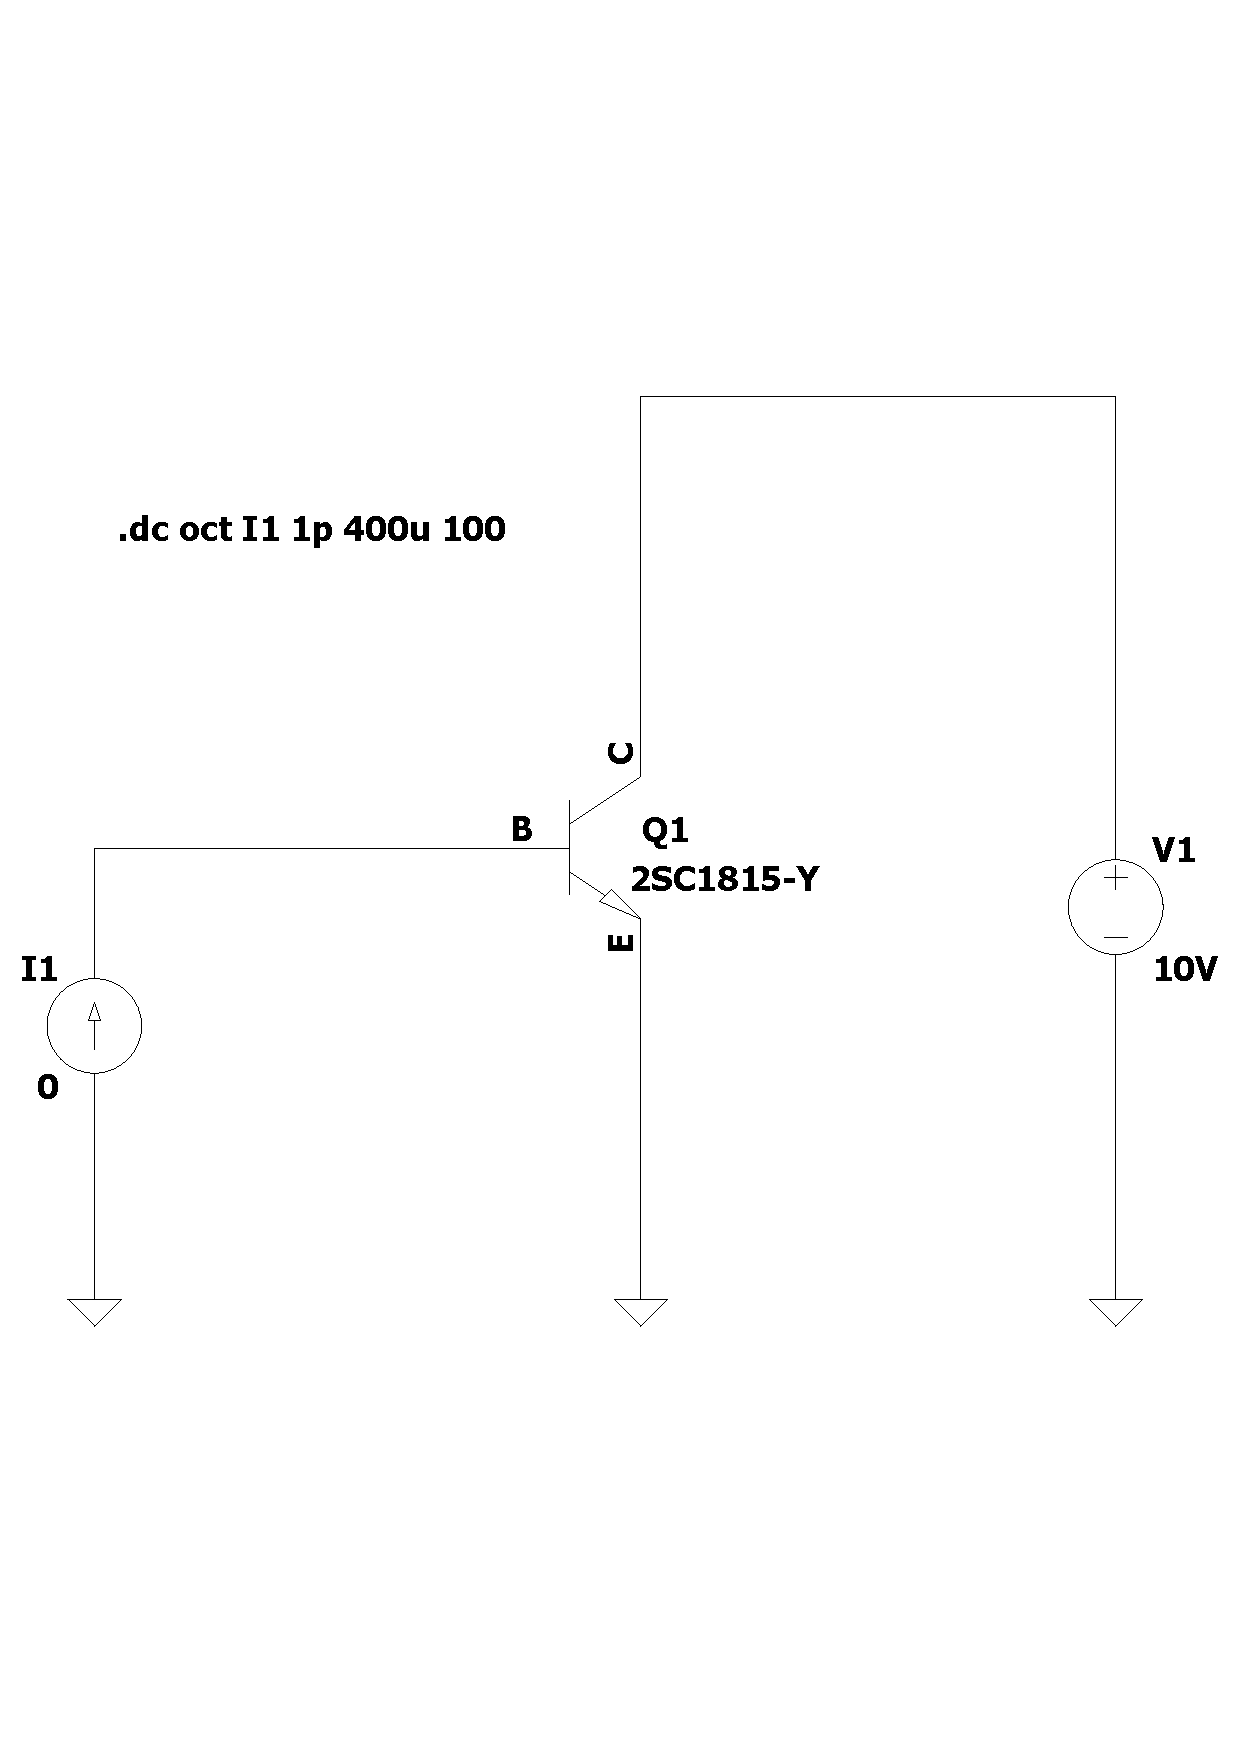
\includegraphics[width=.45\columnwidth]{img/25.pdf}
    }
    \subfigure[dcディレクティブタブ]{
    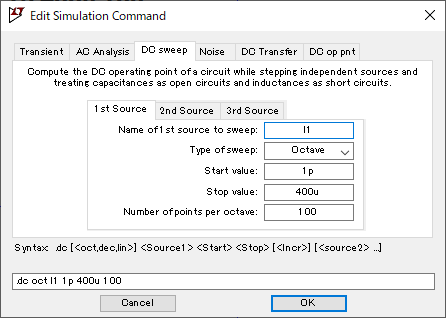
\includegraphics[width=.45\columnwidth]{img/26.png}
    }
    \subfigure[DC動作点解析]{
    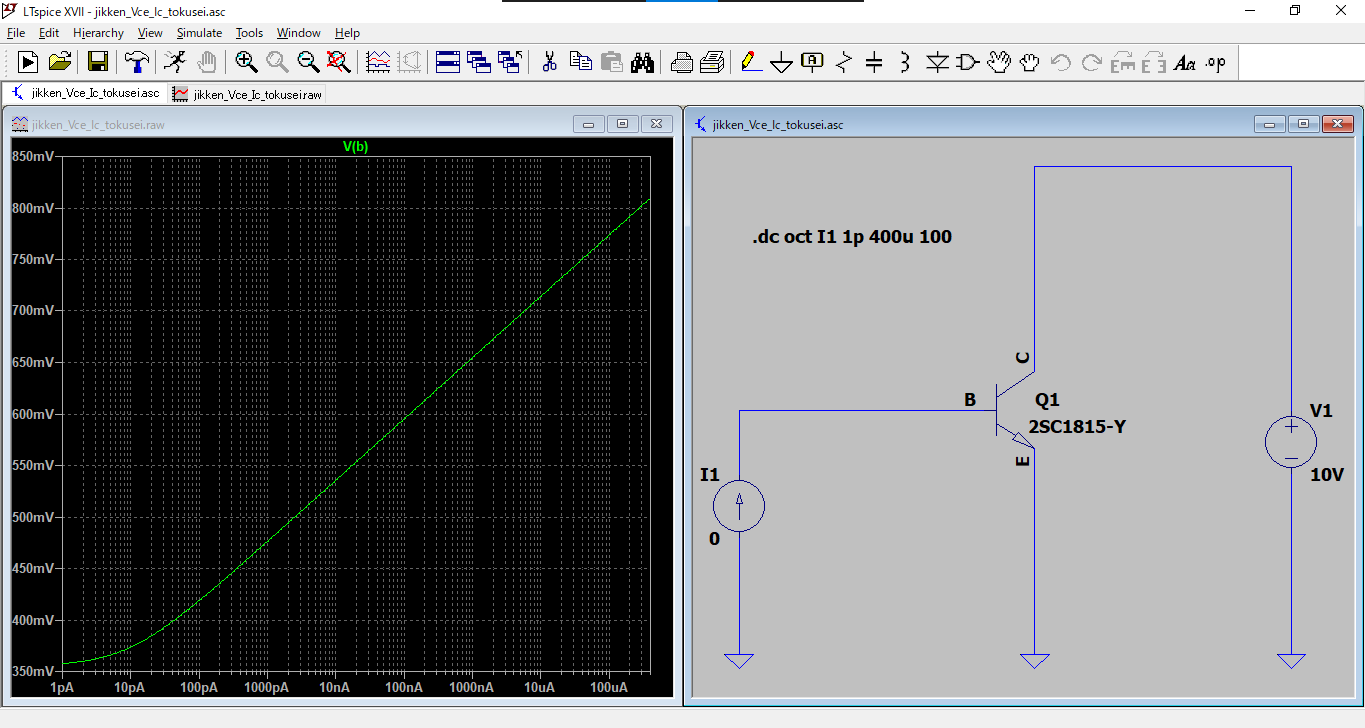
\includegraphics[width=.45\columnwidth]{img/27.png}
    }
    \caption{コントロールパネルの設定} 
    \end{center}
  \end{figure}
  \item 「Run」ボタンをクリックして解析を実行する
  \item ベース電圧を測定する(プローブカーソルを合わせてクリックする)
\end{enumerate}

\subsubsection{$I_E$-$V_{BE}$特性}
$I_E$-$V_{BE}$特性を図に示す。
\begin{enumerate}
  \setlength{\parskip}{0cm} % 段落間
  \setlength{\itemsep}{0cm} % 項目間
  \item グラフの横軸にマウスカーソルを当てて定規カーソルで右クリック →「Horizontal Axis」→ 「Quantity Plotted」欄を "V(b)" に変更 → OKボタンクリックで終了。
  \item グラフの凡例のV(b)をクリック →「Expression Editor」→ 「Enter an algebraic expression to plot」を "-Ie(Q1)" に変更する。
  \item OKボタンをクリックして終了すると -Ie(Q1) vs V(b) のグラフが表示される。
  \item グラフの軸上で右クリックし、「Horizontal Axis」「Vertical Axis」「tick」を調整する。
  \begin{figure}[htb]
    \begin{center}
    \subfigure[$I_E$-$V_{BE}$特性(ダイオード特性)]{
    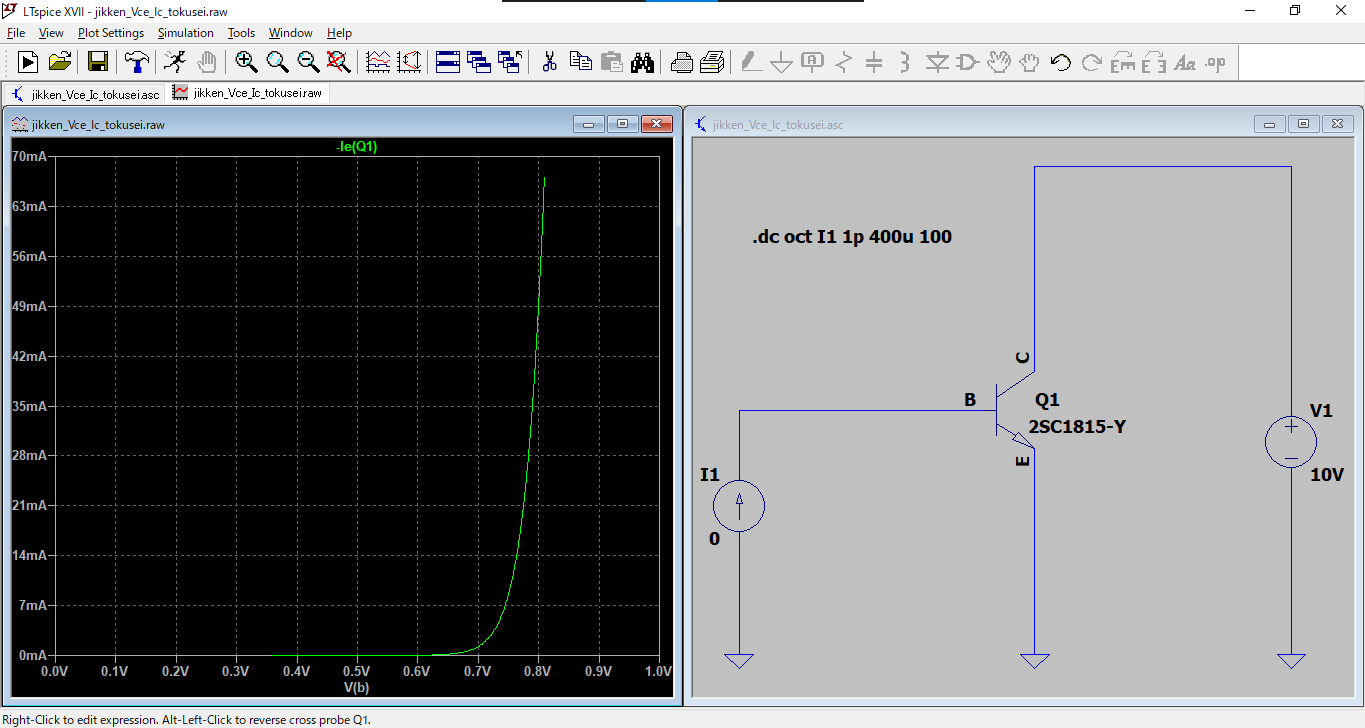
\includegraphics[width=.45\columnwidth]{img/28.png}
    }
    \subfigure[対数表示]{
    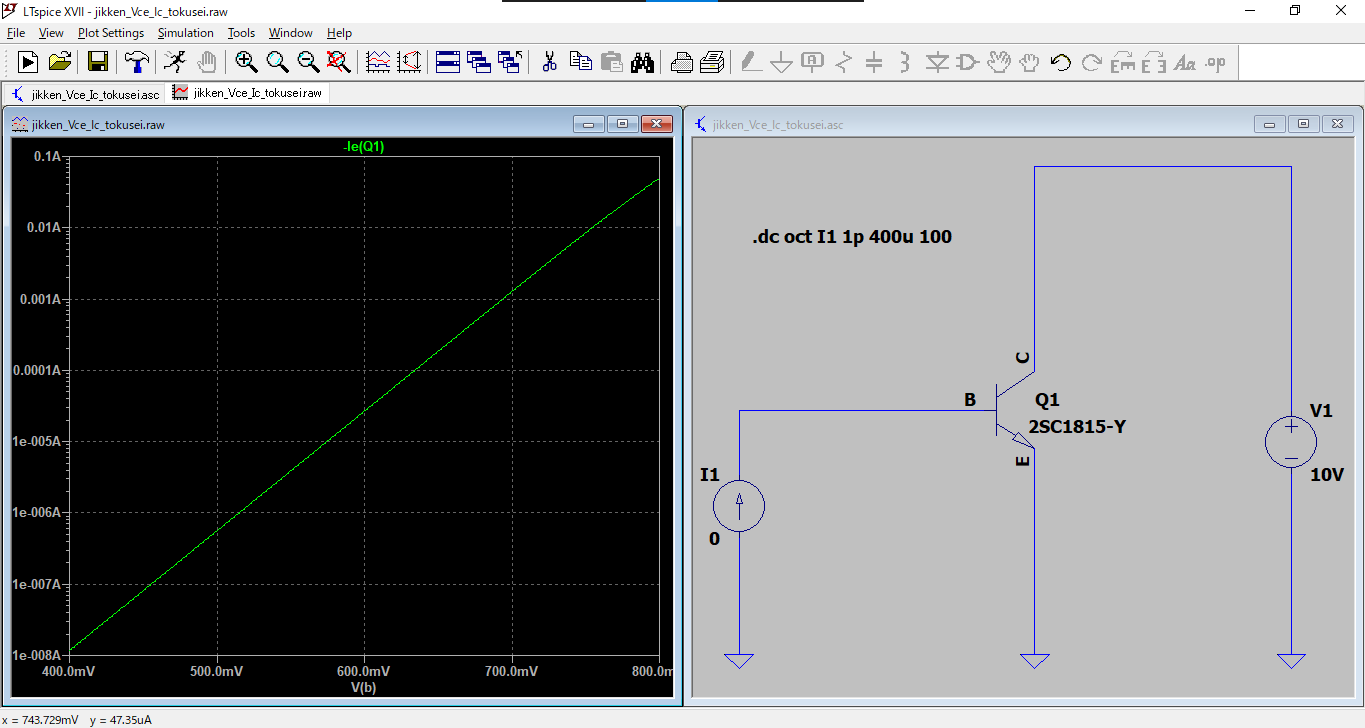
\includegraphics[width=.45\columnwidth]{img/29.png}
    }
    \caption{$I_E$-$V_{BE}$特性}
    \end{center}
  \end{figure}
  \item この特性を印刷するか画像で保存しておく。この回路図も保存しておく。
  \item 「Vertical Axis」→「Logarithmic」欄にチェック → OKと設定すると、片対数グラフでエミッタ電流が直線的に変化している。
\end{enumerate}

\begin{description}
  \setlength{\parskip}{0cm} % 段落間
  \setlength{\itemsep}{0cm} % 項目間
  \item[課題4] 片対数グラフを用いて、$\frac{q}{kT}\log_{10}(e)$の値(理論値)と比較してください。\\
  カーソルを用いて傾きを求める。グラフ上部の凡例を右クリック →「Expression Editor」→「Attached Cursor」→ 1st \verb|&| 2nd を選んで十字カーソルを2個表示
\end{description}

\subsubsection{$I_C$-$I_B$特性}
$I_E$-$V_{BE}$特性を図に示す。
\begin{enumerate}
  \setlength{\parskip}{0cm} % 段落間
  \setlength{\itemsep}{0cm} % 項目間
  \item 「Edit Simulation Cmd」→ 「Edit Simulation Command」→「DC sweep」で以下のように設定しディレクティブを貼り付ける。
  \begin{figure}[htb]
    \begin{center}
    \subfigure[DCスイープ設定]{
    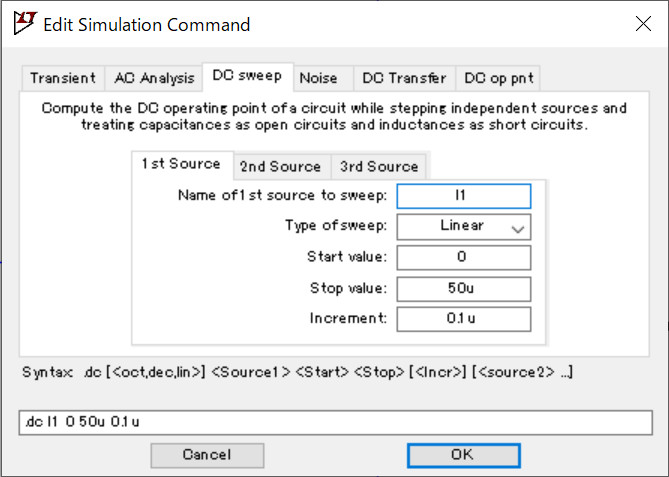
\includegraphics[width=.45\columnwidth]{img/30.png}
    }
    \subfigure[$I_C$-$I_B$特性の]{
    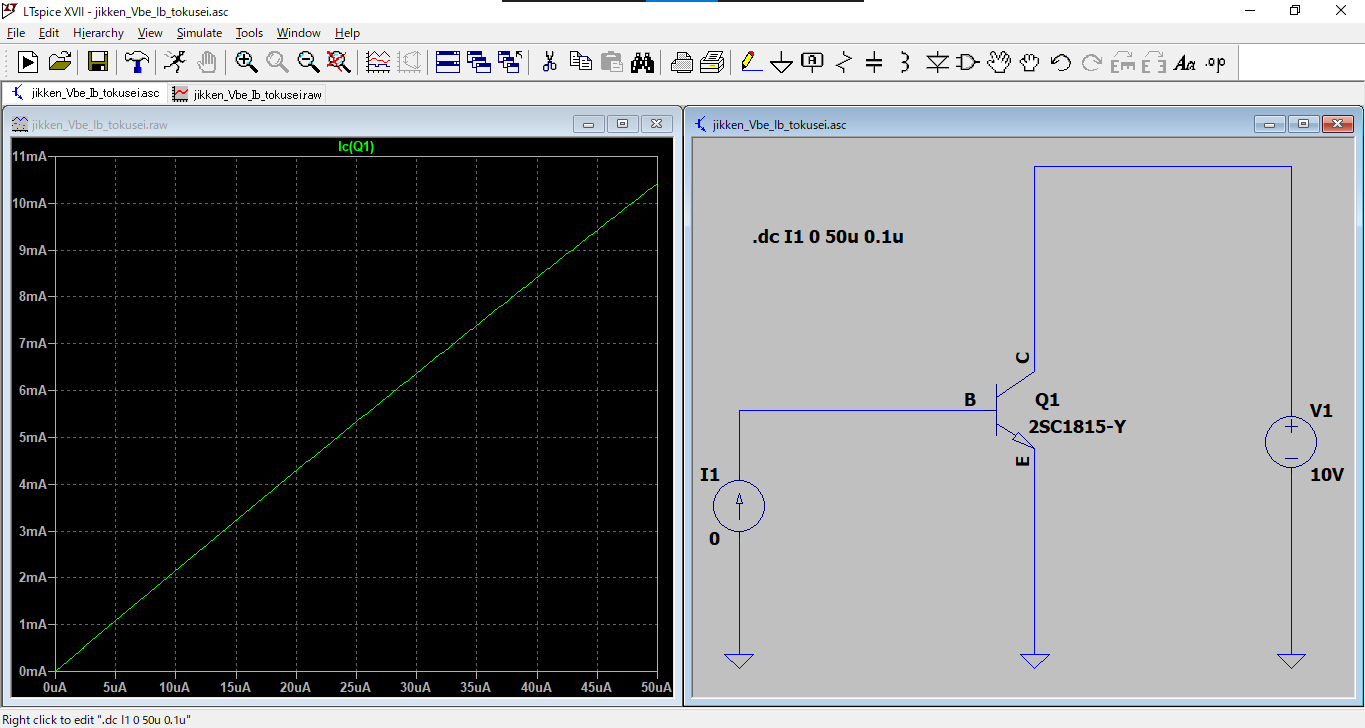
\includegraphics[width=.45\columnwidth]{img/31.png}
    }
    \caption{$I_C$-$I_B$特性}
    \end{center}
  \end{figure}
\end{enumerate}

\begin{description}
  \setlength{\parskip}{0cm} % 段落間
  \setlength{\itemsep}{0cm} % 項目間
  \item[課題5] 実験 $I_C-I_B$ 特性を用いてエミッタ交流電流増幅率と接地直流電流増幅率を求めて下さい。その値を直流電流増幅率と比較して下さい。
  \item[交流電流増幅率] 特性曲線の1点で、ベース電流とコレクタ電流の増幅率を求める。
  \item[直流電流増幅率] 特性曲線の2点で、ベース電流とコレクタ電流の増幅率を求める。
\end{description}

\subsubsection{$I_C$-$V_{CE}$特性}
$I_C$-$V_{CE}$特性を図に示す。
\begin{enumerate}
  \setlength{\parskip}{0cm} % 段落間
  \setlength{\itemsep}{0cm} % 項目間
  \item $I_1$をパラメータとして設定する。$I_1$を右クリックして \verb|"{IB}"| と入力する。
  \item spiceディレクティブを設定
    \begin{itemize}
      \item 「SPICE Directive」(.op) → 「Edit Text on the Schematic」→ 入力欄で右クリック「Help me Edit」→ 「.step Command」→ 「.step Statement Editor」にSPICEディレクティブを書き込む → OK
      \item \verb|.step param IB list 10u 15u 20u 25u 30u 35u 40u 45u 50u| と入力

    \begin{figure}[htbp]
      \begin{center}
      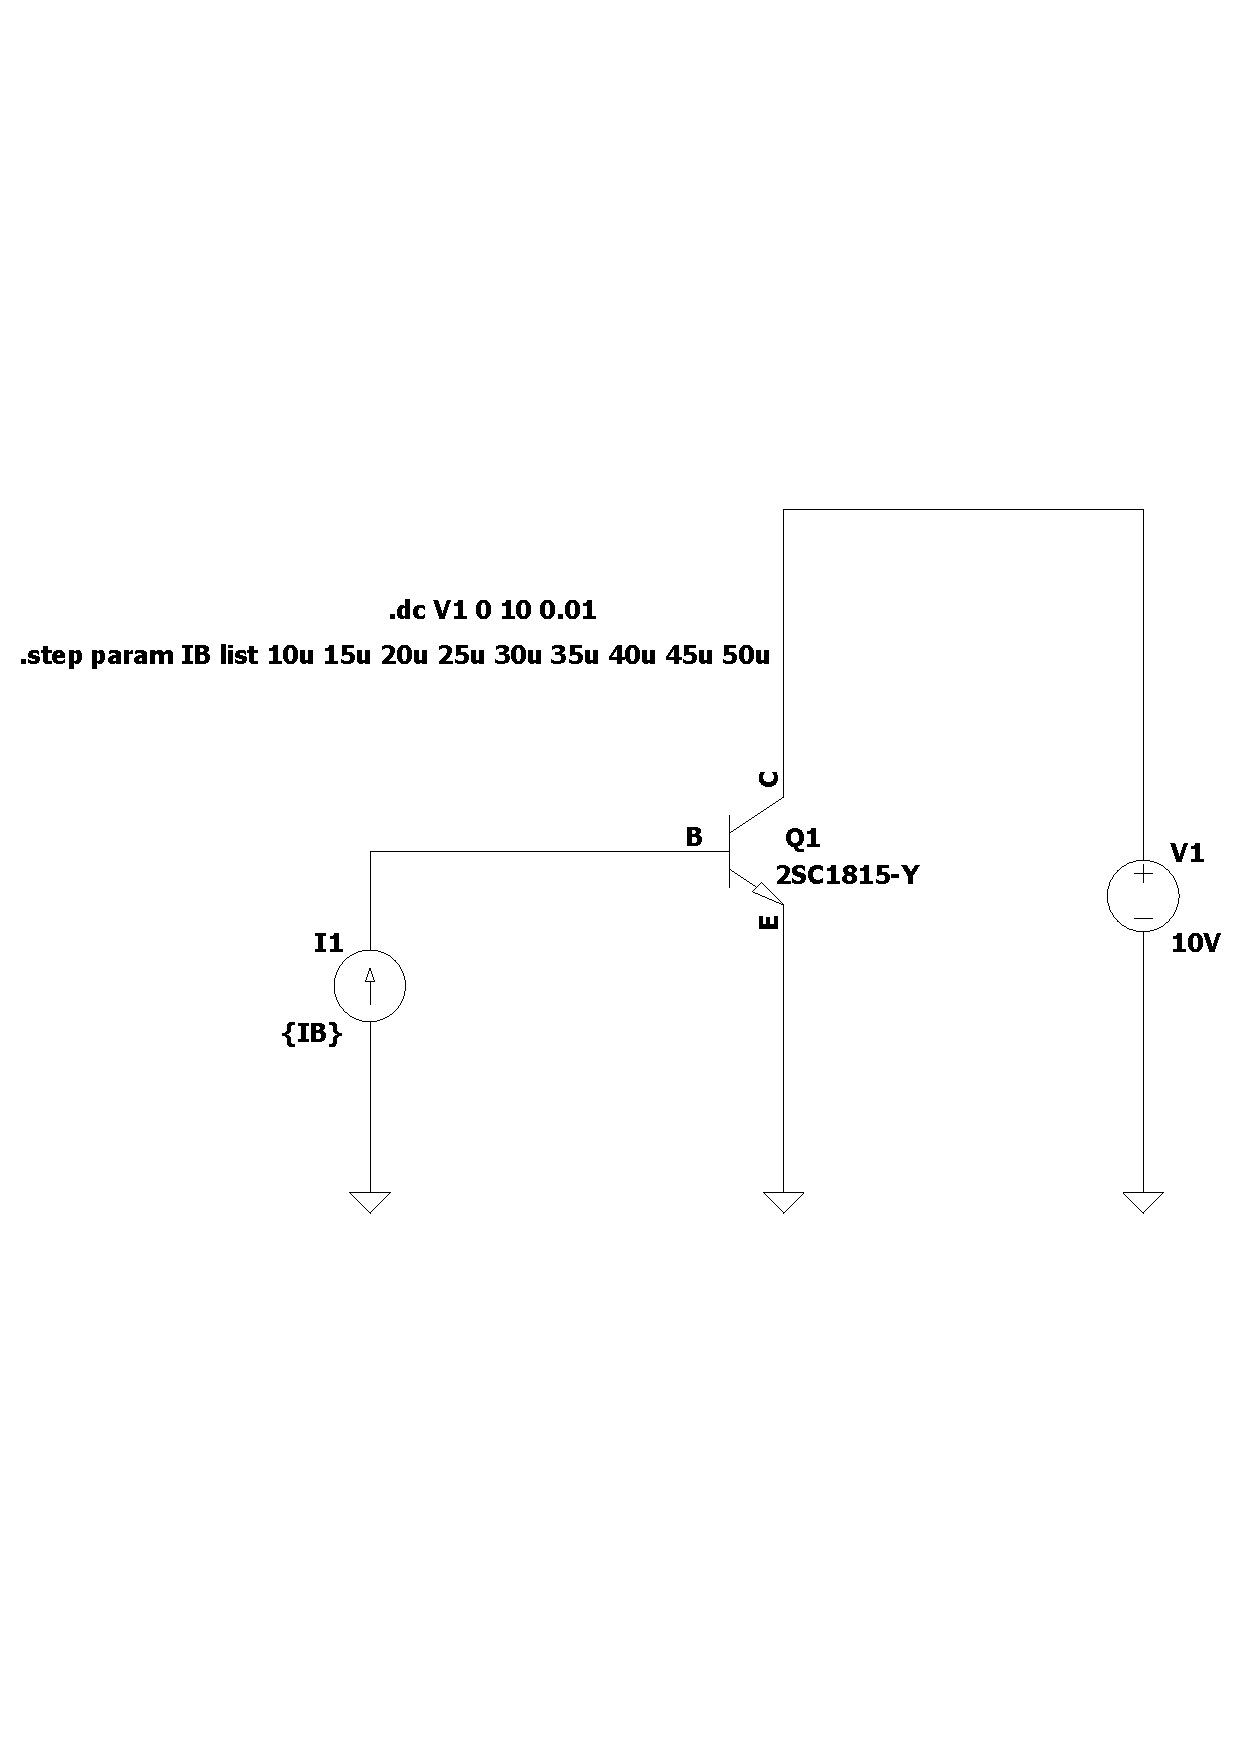
\includegraphics[width=.8\linewidth]{img/32.pdf}
      \caption{$I_C$-$V_{CE}$特性}
      \end{center}
    \end{figure}

    \begin{figure}[htb]
      \begin{center}
      \subfigure[.op ディレクティブ]{
      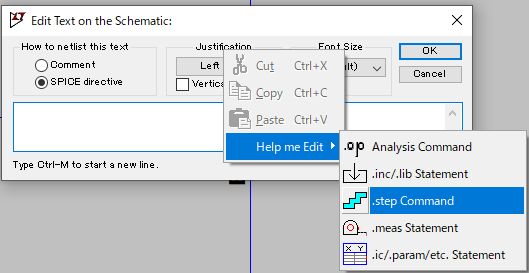
\includegraphics[width=.45\columnwidth]{img/33.png}
      }
      \subfigure[stepパラメータの設定]{
      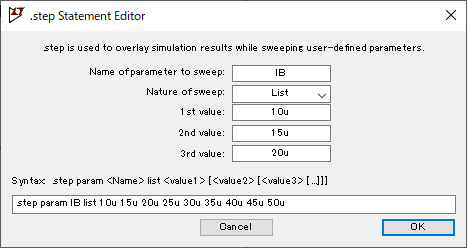
\includegraphics[width=.45\columnwidth]{img/34.png}
      }
      \caption{.op ディレクティブの設定}
      \end{center}
    \end{figure}
  \end{itemize}
  \item DCスイープの設定
  \begin{itemize}
    \item \verb|.dc V1 0 10 0.01|
    \item 「Run」をクリックし、$I_C$をプローブで測る。
  \end{itemize}
  \begin{figure}[htb]
    \begin{center}
    \subfigure[$I_C$-$V_{CE}$特性のディレクティブ]{
    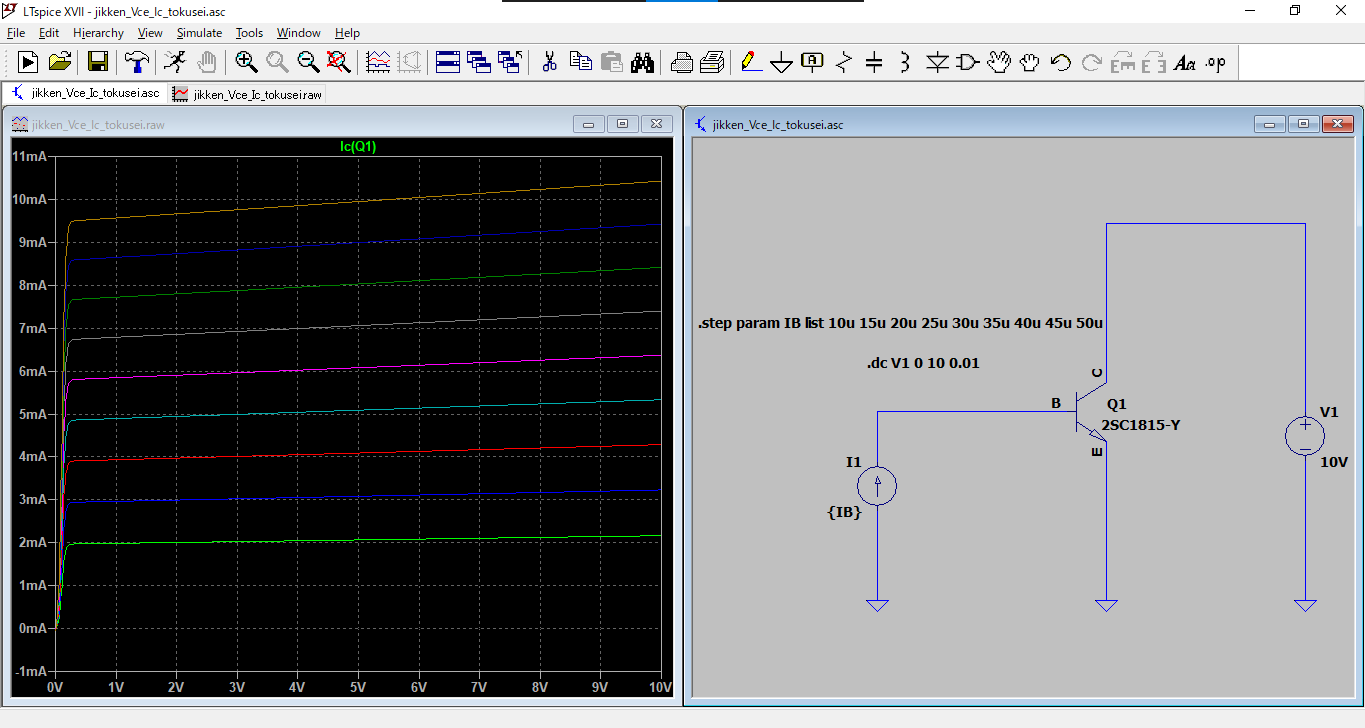
\includegraphics[width=.45\columnwidth]{img/35.png}
    }
    \subfigure[$I_C$-$V_{CE}$特性]{
    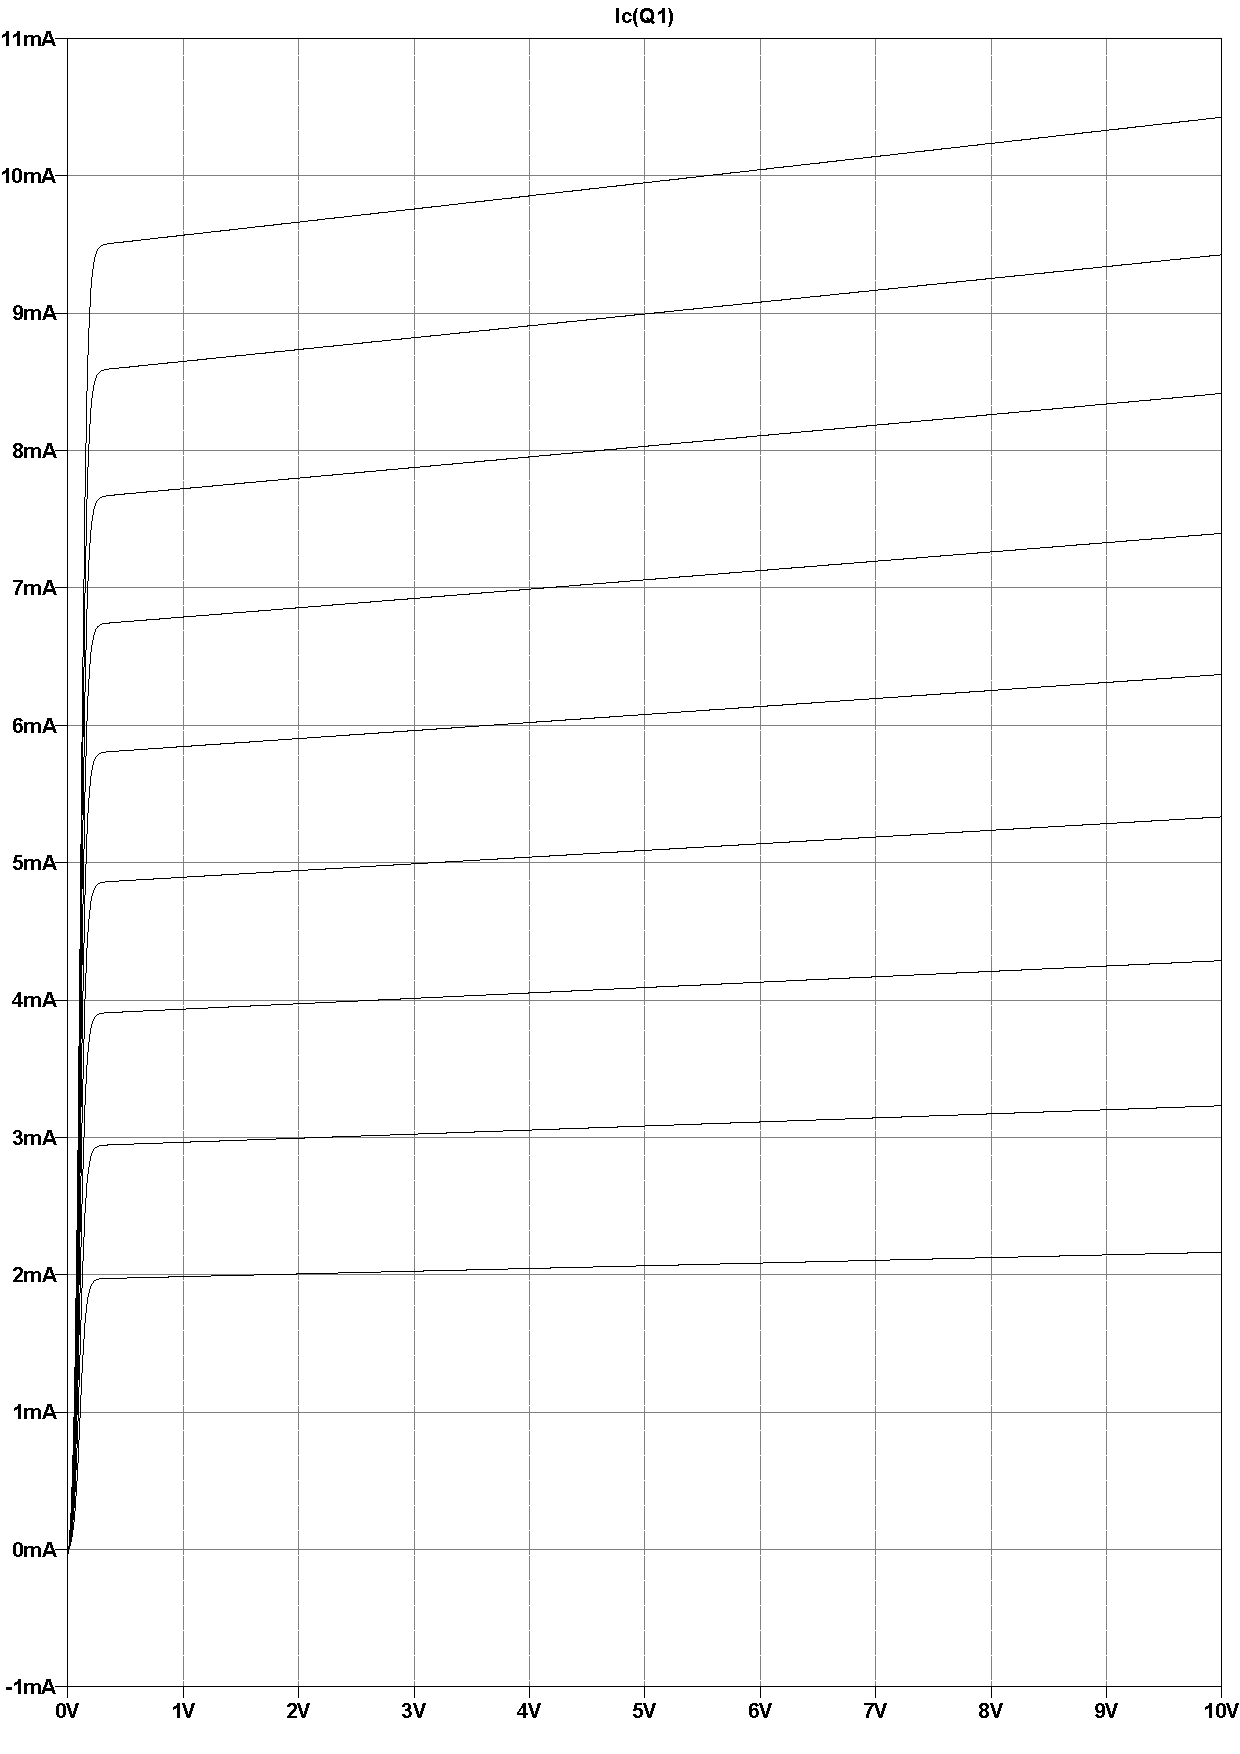
\includegraphics[width=.35\columnwidth]{img/36.pdf}
    }
    \caption{$I_{CE}$-$V_{CE}$特性}
    \end{center}
  \end{figure}
    \item この特性を印刷するか画像で保存しておく。
    \begin{description}
      \setlength{\parskip}{0cm} % 段落間
      \setlength{\itemsep}{0cm} % 項目間
      \item[課題6] $I_C-V_{CE}$ 特性から、入力信号トランジスタの増幅回路を設計するための$V_{CE}$の領域は何 V \verb|～| 何 V が良いでしょうか？
    \end{description}
\end{enumerate}
\section{エミッタ接地回路のバイアス電圧$v_{be}$の設定}
エミッタ接地回路の動作点設定について原理の説明とシミュレーションによる演習を並行して行うことで理解する。

\begin{description}
  \setlength{\parskip}{0cm} % 段落間
  \setlength{\itemsep}{0cm} % 項目間
  \item[ゴール] 2電源バイアス回路をLTSpiceで設計する。(バイアス電圧Vbeと負荷抵抗Rlを決定する。)
  \item[キーワード] $I_C$-$V_{CE}$特性、$I_E$-$V_{BE}$ 特性、負荷線、動作点 $V_{CEO}$・$I_{CO}$・$V_{BEO}$
  \item[ストーリー] $I_E$-$V_{BE}$特性と、$I_C$-$V_{CE}$特性を使って、動作点 $V_{CEO}$・$I_{CO}$・$V_{BEO}$ を決める。→ 過渡解析により増幅率を実測 → 計算値と比較。
\end{description}

\subsection{原理・計算}
エミッタ接地増幅回路の基本原理を下図に示す。
\begin{figure}[htb]
  \begin{center}
  \subfigure[エミッタ接地回路の原理図]{	% 副題なし
  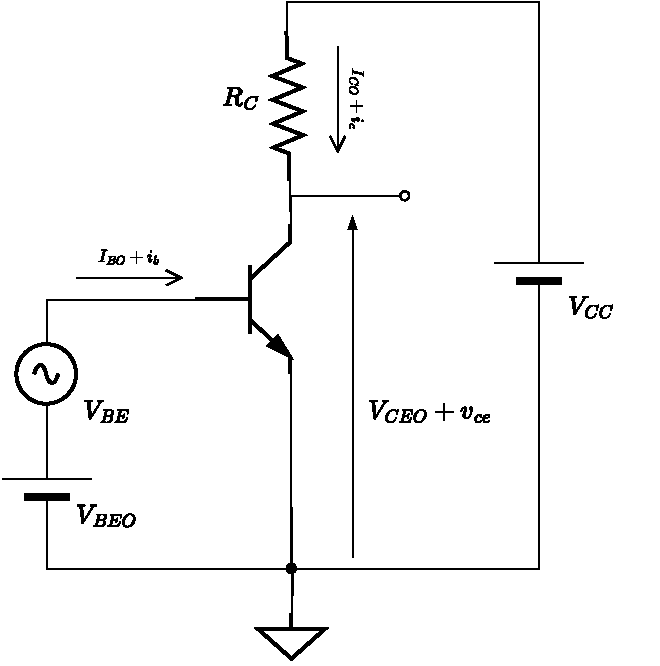
\includegraphics[width=.33\columnwidth]{img/37.pdf}
  }
  \subfigure[$V_{BE}$-$I_E$特性]{
  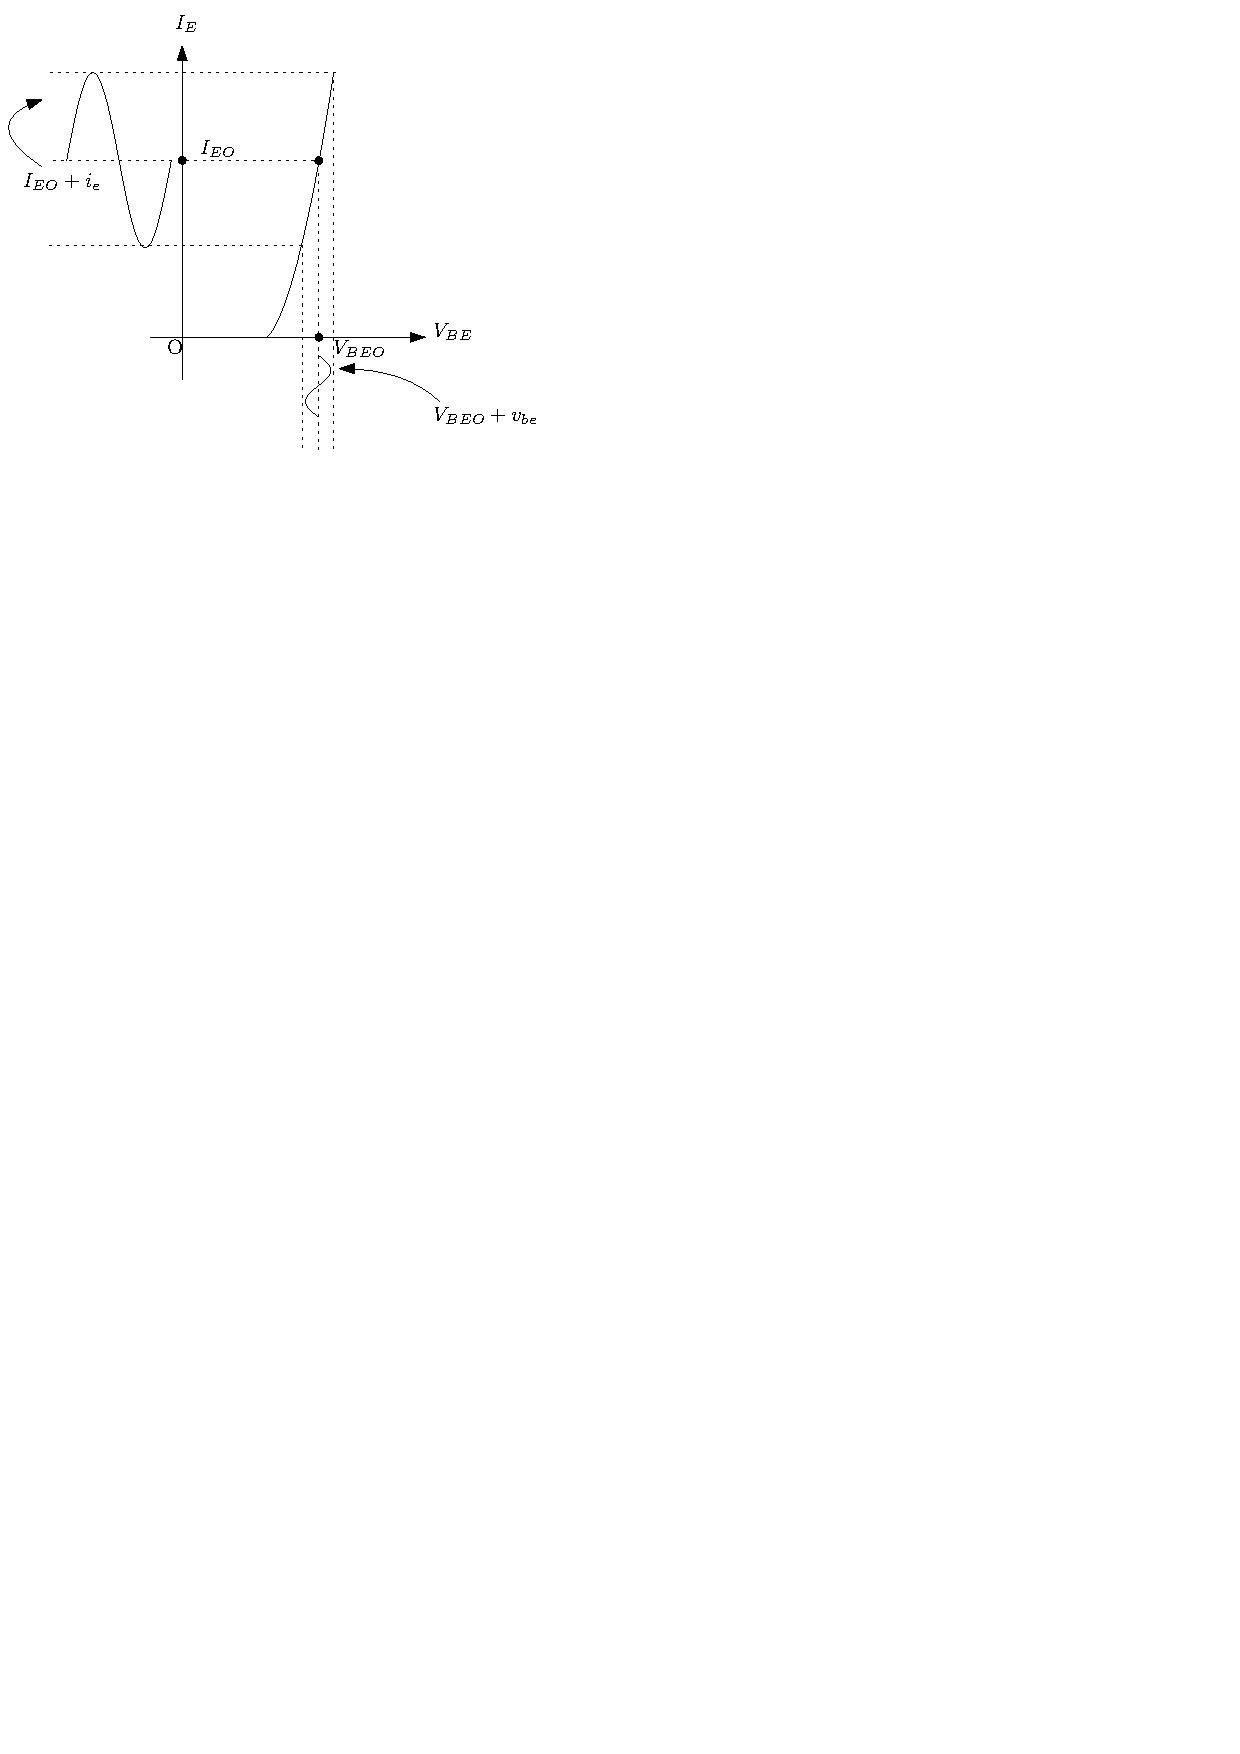
\includegraphics[width=.33\columnwidth]{img/38.pdf}
  }
  \subfigure[$I_C$-$V_{CE}$特性]{
  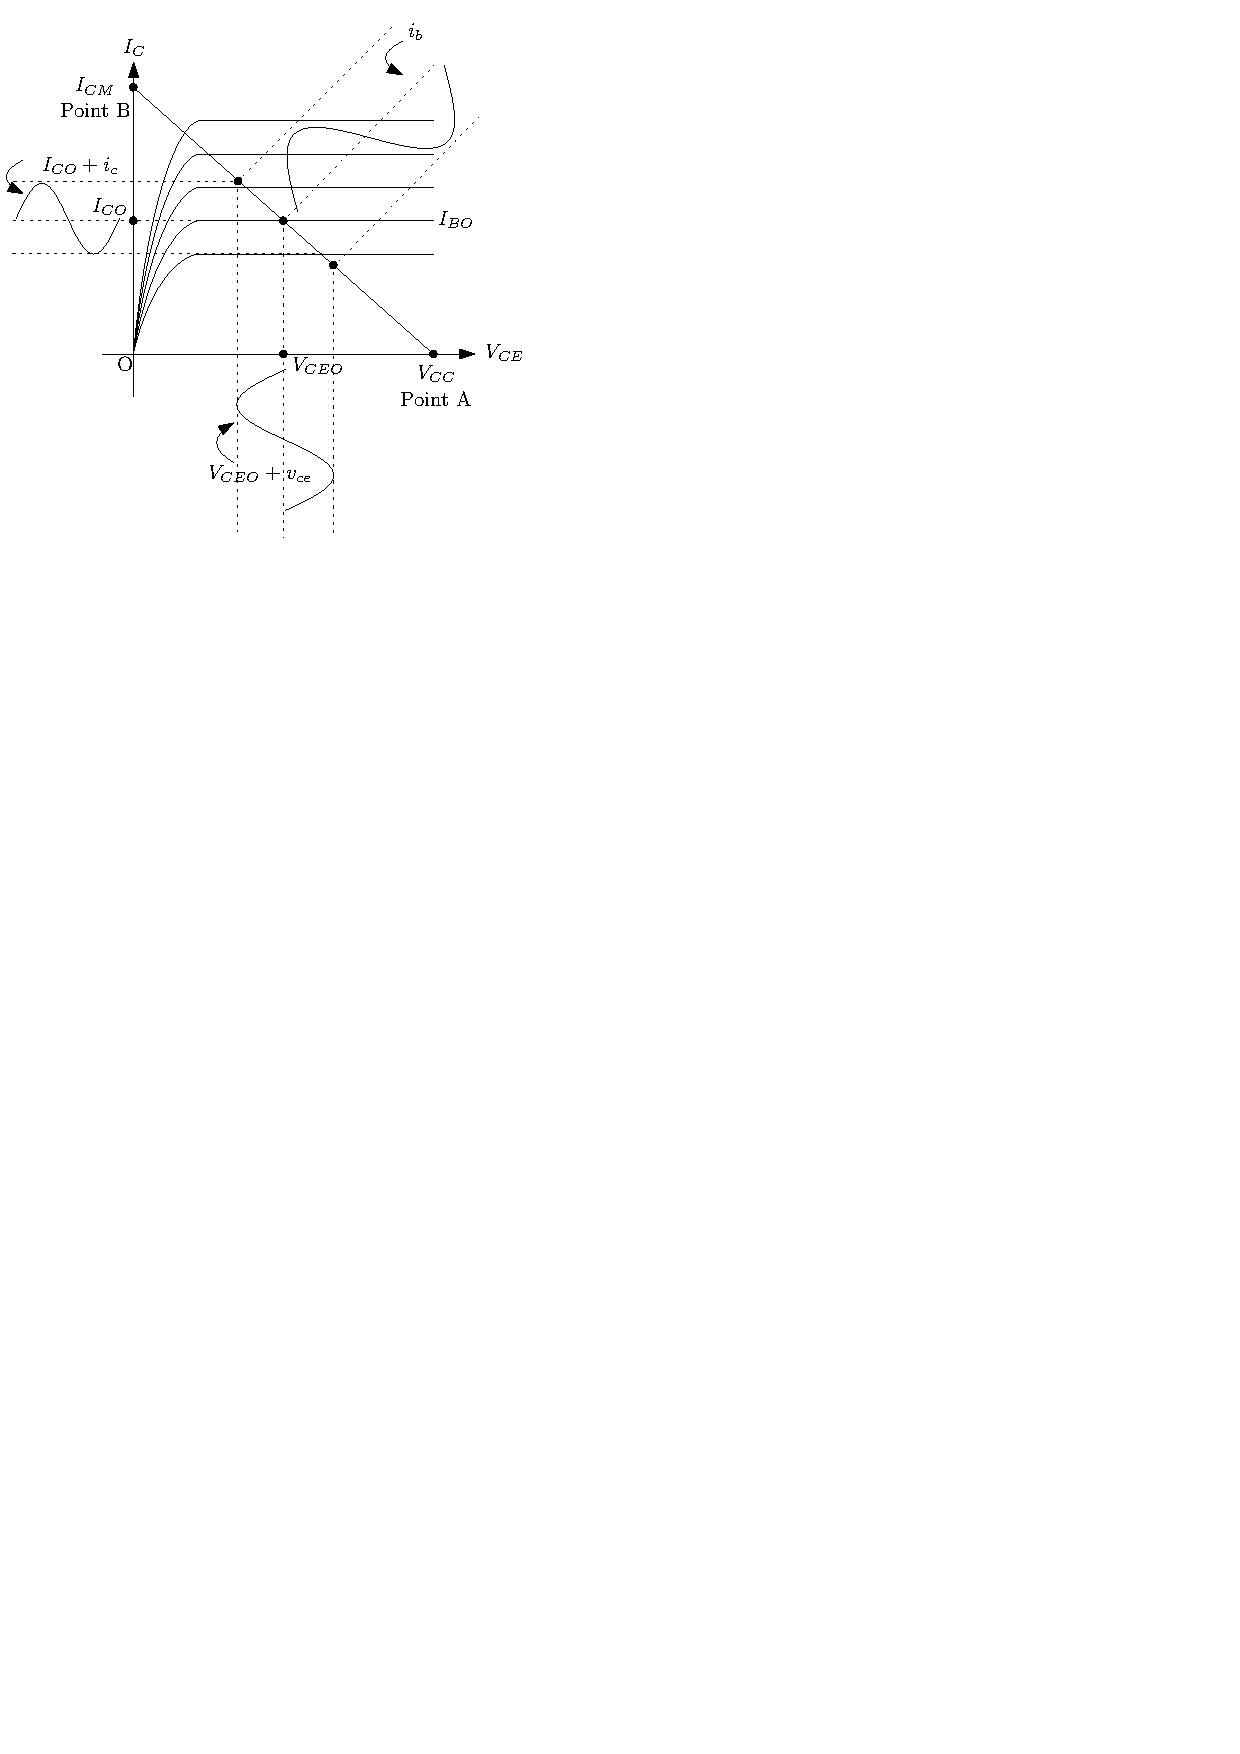
\includegraphics[width=.33\columnwidth]{img/39.pdf}
  }
  \caption{エミッタ接地回路の基本原理} 
  \end{center}
\end{figure}

\begin{enumerate}
  \setlength{\parskip}{0cm} % 段落間
  \setlength{\itemsep}{0cm} % 項目間
  \item バイアス電圧 $V_{BEO}$ を印加
  \item 交流電圧 $v_{be}$ を加えると、ベース電流は、動作点 $I_{BO}$ を中心に $i_b$ 変化する
  \item コレクタ電流は動作点 $I_{CO}$ を中心に $i_c$ 変化する。
  \item コレクタ-エミッタ間電圧は、動作点 $V_{CEO}$ を中心に $v_{ce}$ 変化する
\end{enumerate}
\subsection{バイアス電圧$V_{BE}$の設計手順}
\begin{enumerate}
  \setlength{\parskip}{0cm} % 段落間
  \setlength{\itemsep}{0cm} % 項目間
  \item $I_C$-$V_{CE}$ 特性に負荷線を引く (\textbf{$R_C$ を決める})\\
  $V_{CC}$、$I_{CM}$ は自分で決める。\\
  $V_{CC} = 10$ V $I_{CM} = 11$ mA として計算\\
  $V_{CE} = 0$ の時、($v_{ce}$ を短絡)$I_{CM} = \frac{V_{CC}}{R_C}$\\
  -$I_C = 0$ の時、($R_C$ で電圧降下が起きない。$R_C$ を短絡) $V_{CEM} = V_{CC}$\\
  $$V_{CC} = \frac{10}{R_C}  より、 \frac{V_{CC}}{R_C} = I_{CM} = \frac{10}{R_C} = 11 \textrm{mA}$$
  $$よって、R_C = 909.0909 \Omega$$\\
  $(0, \frac{V_{CC}}{R_C})$、$(V_{CC}, 0)$を通る直線は、
  $$I_C = - \frac{1}{R_C} V_{CE} + \frac{V_{CC}}{R_C} = \frac{10 - V_{CE}}{909.09}$$
  \item $V_{CE}$ の動作点 $V_{CEO}$ を求める ($v_ce$ は自分で決める。±の値になる)\\
  コレクタエミッタ間電圧 $V_{CE}$ の振幅が大きく取れるように動作点を設定する。\\
  エミッタ接地回路では、コレクタエミッタ間電圧 $V_{CE}$ の動作点は電源電圧 $V_{CC}$ と 0 V
  の真ん中付近に $V_{CEO}$ を設定する。
  今回は、$V_{CC} = 10$ Vであるため、$V_{CEO} = \frac{V_{CC}}{2} = 5\textrm{V}$を動作点とする。
  また、今回は$v_{ce} = \pm 0.9$ Vとして計算する。
  \item コレクタ電流 $i_c$ の動作点 $I_{CO}$ を求める。\\
  $I_C-V_{CE}$ 特性で、$V_{CEO}$ を決めたとき、その振れ幅に対応する $i_c$ と、$V_{CEO}$ に対する、$I_{CO}$ (コレクタ電流の動作点)が決まる。($I_{CO}$が決まると、$I_{BO}$が決まる。)
  $$I_{CO} = \frac{V_{CC}}{2R_C} = \frac{V_{CEO}}{R_C} = \frac{5}{909.09} \approx 5.5 \textrm{mA}$$
  $V_{CE} = 5 - 0.9 = 4.1$ Vの場合、$I_C \approx 6.49$ mA\\
  $V_{CE} = 5 +0.9 = 5.9$ Vの場合、$I_C \approx 4.51$ mA\\
  $I_C$の振れ幅は、$6.49 - 4.51 = 1.98$ mAであるため、
  $I_C = I_{CO}+i_c = 5.5 \pm 0.99$ mAと決まる。
  \item ベースエミッタ間電圧 $V_{BE}$ の動作点 $V_{BEO}$ を求める\\
  $I_C \approx I_E$ とし、LTSpiceでシミュレーションした$I_E-V_{BE}$ 特性の値をカーソルで読み取る。\\
  $I_C = 5.5 + 0.99$ mA の場合、$I_E-V_{BE}$ 特性より $V_{BE} = 0.7427$ V\\
  $I_C = 5.5 - 0.99$ mA の場合、$I_E-V_{BE}$ 特性より $V_{BE} = 0.73365$ V\\
  $I_C = I_{CO} = 5.5$ mA の場合、$V_{BEO} = 0.7386$ V
\end{enumerate}

\subsection{LTspiceで演習}
計算した値を用いて、下記回路図を設計する。なお、入力信号は正弦波信号$v_{be} = 5.27$ mV を使用している。

\begin{figure}[htbp]
  \begin{center}
  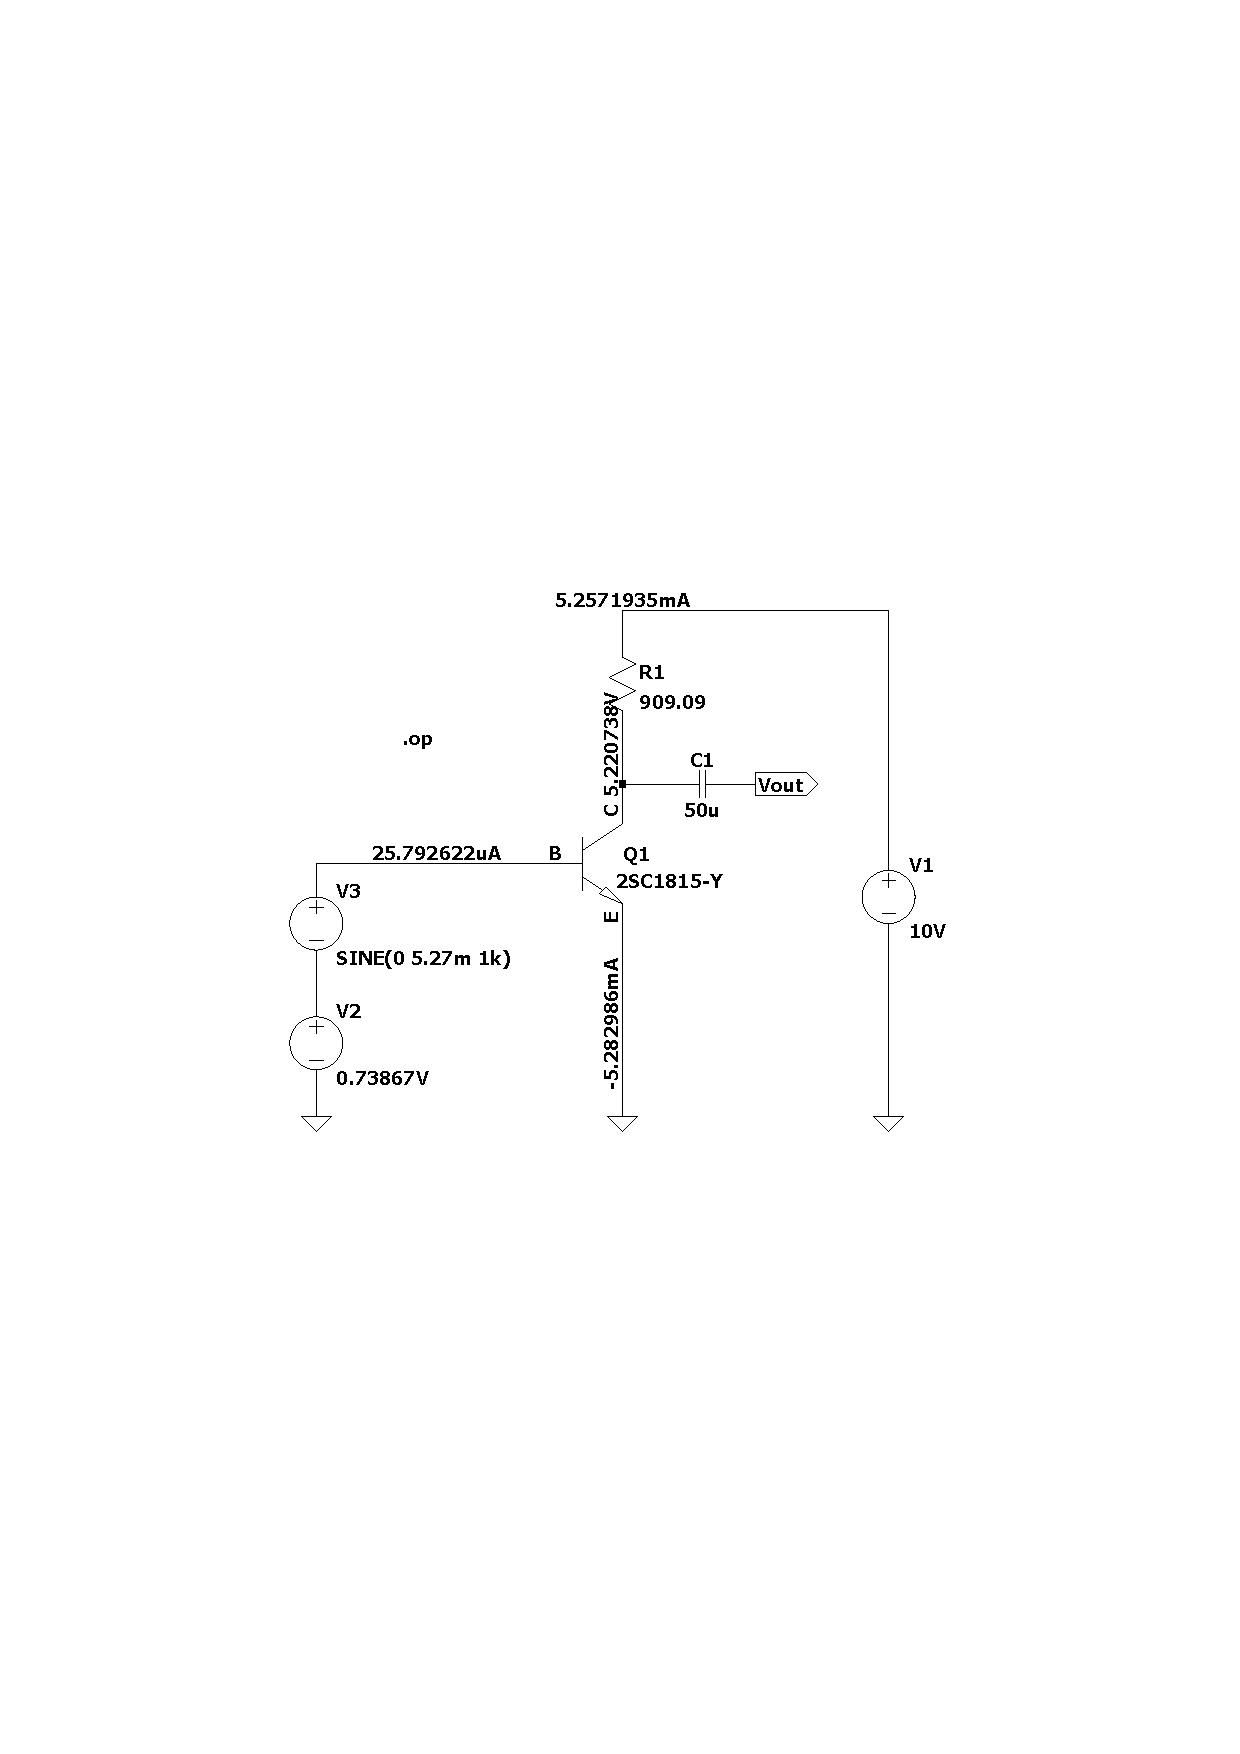
\includegraphics[width=.8\linewidth]{img/40.pdf}
  \caption{2電源バイアス回路の動作点}
  \end{center}
\end{figure}

\subsubsection{DC動作点解析}
spiceディレクティブ「DC op pnt」に ".op" のみ記述し、ディレクティブに張り付ける → 「Run」で実行。→ 設計した値に対応するベース電流、コレクタ電流がDC動作点の解析結果として現れる。
\begin{figure}[htbp]
  \begin{center}
  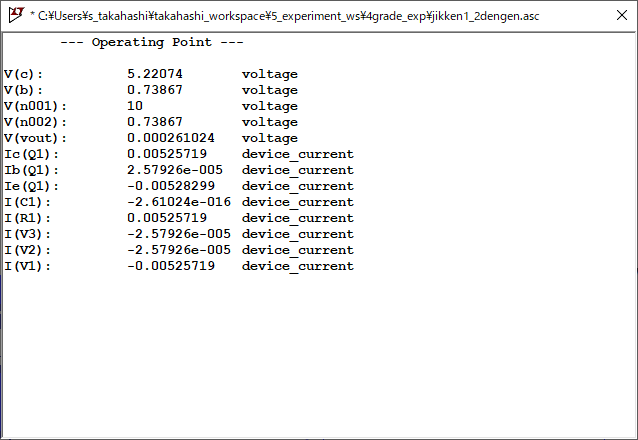
\includegraphics[width=.5\linewidth]{img/41.png}
  \caption{動作点解析結果}
  \end{center}
\end{figure}

\begin{description}
  \setlength{\parskip}{0cm} % 段落間
  \setlength{\itemsep}{0cm} % 項目間
  \item[課題7] ベース電流、コレクタ電流のDC動作点をシミュレータの結果で確認して下さい。
  それらの値を用いて、直流電流増幅率$\beta_0$を求めて、計算値と比較して下さい。
\end{description}

\subsubsection{過渡解析}
「Edit Simulation cmd.」から Transient 解析を選び、「.tran 3ms」ディレクティブを適用させて、過渡解析を実行する。
この時、$V_C、I_C、I_B$ の波形を確認する。

\begin{figure}[htbp]
  \begin{center}
  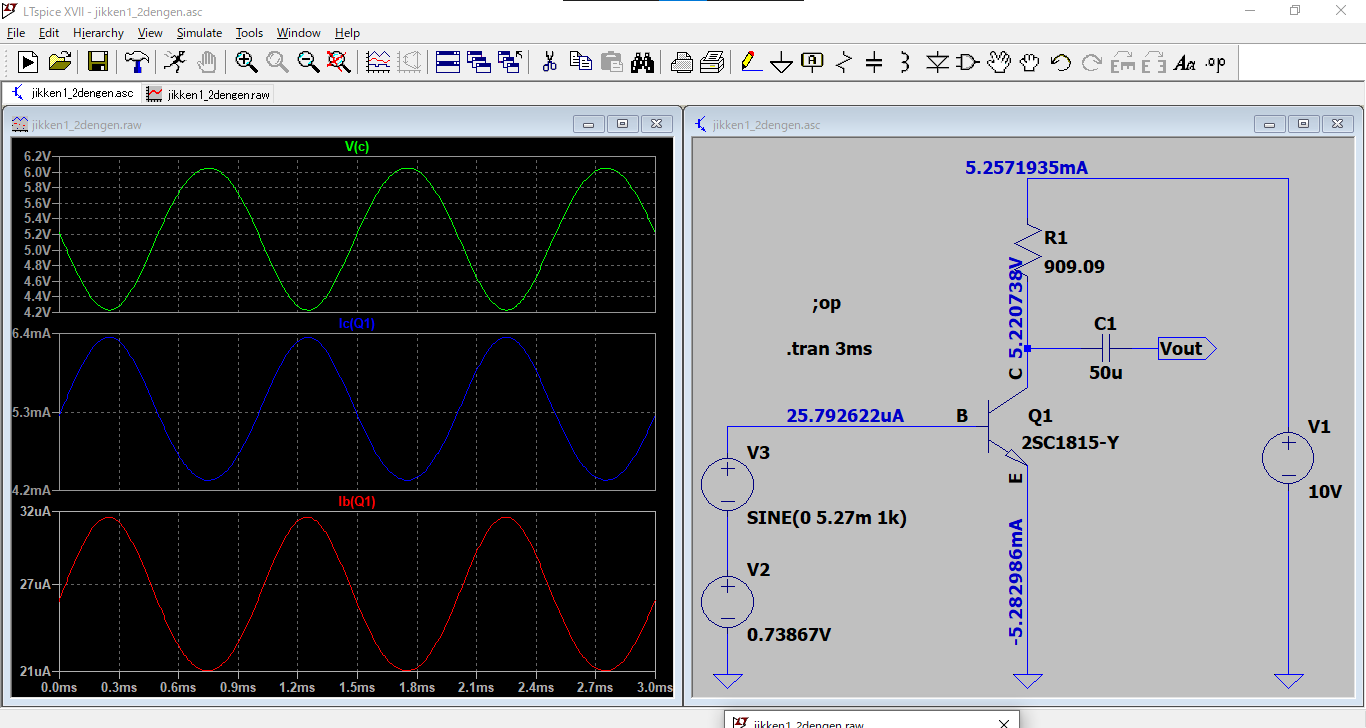
\includegraphics[width=0.7\linewidth]{img/42.png}
  \caption{過渡解析結果}
  \end{center}
\end{figure}

\begin{description}
  \setlength{\parskip}{0cm} % 段落間
  \setlength{\itemsep}{0cm} % 項目間
  \item [課題8] 過渡解析を実行した際の波形の値を説明して下さい。
  (動作点が正しく設定されているかどうか、波形がこの値をとる理由を考えて下さい。)\\
  \item [課題9] 交流電流増幅率 $\beta_0$ を求めて下さい。($\beta_0 = i_c/i_b$)
\end{description}
\section{電流帰還バイアス回路の動作点設定(直流の話)}
電流帰還バイアス回路は、エミッタ接地増幅回路の基本形であり、増幅回路の直流電流動作点を決めるための動作原理図である。(実際にこの形のままで使われることはない。)
固定バイアス、自己バイアス等、入力信号(電圧)にバイアスを加える方法はいくつかあるが、一般的に、トランジスタの持つ特性により動作に悪影響を受ける。(直流電流増幅率の温度変化)
この回路は、温度変化による影響を受けにくい設計となっている。

\begin{description}
  \setlength{\parskip}{0cm} % 段落間
  \setlength{\itemsep}{0cm} % 項目間
  \item[ゴール] 前章で決めた動作点と諸条件から直流電流の動作点を決める。(ブリーダ抵抗の値を決定する。)
  \item[キーワード] ブリーダ抵抗、温度補償
  \item[ストーリー] 前章で決めた動作点+諸条件 → 閉路方程式を立てて回路に流れる直流電流を求める。→ 直流電流の動作点を決める。→ LTspice上で設計 → DCスイープにより動作点を確認 → 計算値と比較
\end{description}

\subsection{原理・計算}
$V_{CC}$ を $R_1$ と $R_2$ で分圧することで、ベース電位 $V_{BQ}$ を設定する。
添え字 Q がバイアス計算で求める量である。\\

\begin{figure}[htbp]
  \begin{center}
  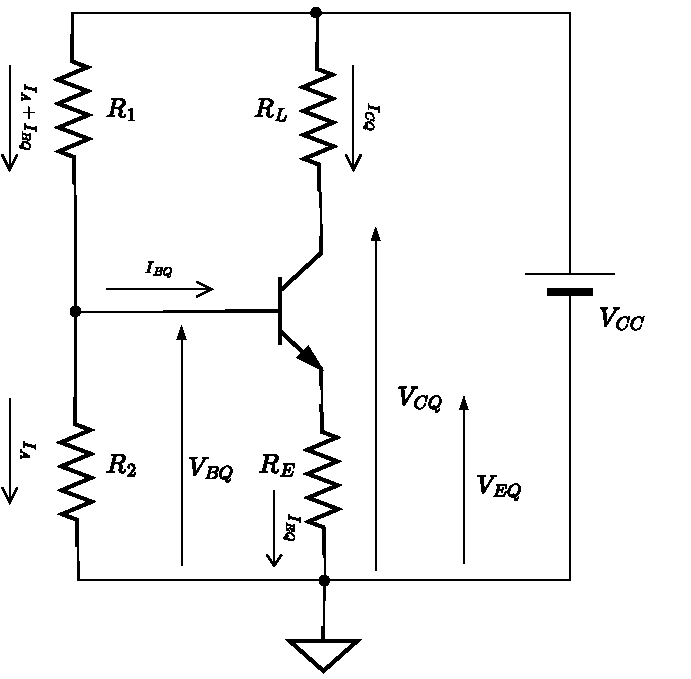
\includegraphics[width=0.45\linewidth]{img/43.pdf}
  \caption{電流帰還バイアス回路の原理図}
  \end{center}
\end{figure}


$I_{BQ} \approx 0$ と近似(他の電流と比べて小さいため)すると、$R_1$ を流れる電流は、全て$R_{2}$ に流れるので、\\
$$V_{BQ} \approx \frac{R_2}{R_1+R_2}V_{CC}$$ により、ベースのバイアス電圧が求まる。ベース電流がゼロなので、$r_b$ による電圧降下はゼロである。(ベース層の抵抗)\\
$I_{EQ} = \frac{V_{EQ}}{R_E}$ ($V_{EQ}$ は $R_E$ の両端電圧)\\
$V_{EQ} = V_{BQ} - V_{BE}$ ($V_{BE}$ は、前のシミュレーションで求めた約 0.7 V の値を使う。)\\
$I_{CQ} \approx I_{EQ} (I_{EQ} = I_{CQ} - I_{BQ} \approx 0)$\\
$V_{CQ} = V_{CC} - R_LI_{CQ}$\\
$I_{BQ} = \frac{I_{CQ}}{\beta_0}$ ($\beta_0$: 直流電流増幅率)

\subsection{回路の特徴}
\begin{enumerate}
  \setlength{\parskip}{0cm} % 段落間
  \setlength{\itemsep}{0cm} % 項目間
  \item 温度補償\\
  トランジスタの直流電流増幅率は、温度によって上昇する性質がある。
  $\beta_{0}$ 増加 → $I_{CQ}$ が増加 → $I_{EQ}$ も増加 → $R_{E}I_{EQ}$ が増加\\
  $V_{BE} = V_{BQ} - V_{CQ}$ より、$V_{BE}$ が減少 → $I_{BQ}$ が減少 → $I_{CQ}$ の増加を抑制する。
  \item 利点: 温度が変化した場合のバイアス安定度が高い。
  \item 欠点: $R_2$ を比較的小さく設定する関係で、これらの抵抗に流れる電流(ブリーダ電流)により、消費電流が大きくなる。
\end{enumerate}

\subsection{電流帰還バイアス回路の設計手順}
電流帰還バイアス回路を設計するためにあらかじめ条件が要求される。
\begin{enumerate}
  \setlength{\parskip}{0cm} % 段落間
  \setlength{\itemsep}{0cm} % 項目間
  \item 諸条件の設定
  \begin{itemize}
    \item 使用するトランジスタ:2SC1815
    \item 直流増幅率$\beta_0 = 213$
    \item $V_{BE} = 0.7386$ V
    \item $V_{CC} = 10$V
    \item バイアス点電流$I_{CO}=5.5$mA
    \item $I_{BO}= \frac{I_{CO}}{\beta_0} = \frac{5.5\times10^{-3}}{213} \approx 25.82 \mu$A
    \item $R_E$による電圧降下は、$V_{CC}$の10\verb|%| とする。
    \item $V_{CEO} = V_{RLO}$とする。
    \item ブリーダ電流$I_A$: $I_{BO}$ の20倍
  \end{itemize}
  \item $R_E$を求める\\
  $V_{EO} = R_EI_{EO} = 0.1V_{CC} = 1.0$ V $I_{EO} \approx I_{CO}$ より
$$R_E = \frac{V_{EO}}{I_{CO}} = \frac{1}{5.5 \times 10^{-3}} \approx 181.818 \Omega$$
  \item $R_L$を求める\\
  $R_L$ に流れる電流 $I_{CO}$ について、$V_{CEO} = V_{CO} -V_{EO}$ と $R_LI_{CO}$ を等しくすると、出力信号の振幅を最大化できる。(動作点を負荷線の真ん中に選ぶ)
  \item ブリーダ電流$I_A$を求める。\\
  $20 \times I_{BO} = 20 \times 25.82 \mu$ A $= 0.5164$ mA
  \item $R_2$を求める\\
  $V_{BO} = R_2I_A$ より、$$R_2 = \frac{V_{BO}}{I_A} = \frac{(V_{EO}+V_{BE})}{I_A} = \frac{(1+0.7386)}{0.5164}\textrm{mA}$$ $$\approx 3366.769946 \approx 3.4 \textrm{k}\Omega$$
  \item $R_1$を求める
  $$R_1 = \frac{(V_{CC} - (V_{EO}+V_{BE}))}{I_A+I_{BO}} = \frac{(10 - (1+0.7386))}{(0.5164 \times 10^{-3} + 25.82\mu)} = 15236.25097 \approx 15.2 \textrm{k}\Omega$$
\end{enumerate}

\subsection{LTspiceで演習}
これらの計算値を用いて回路を設計する。
\subsubsection{DC動作点解析}
\begin{description}
  \setlength{\parskip}{0cm} % 段落間
  \setlength{\itemsep}{0cm} % 項目間
  \item [課題10] 以下の回路を作成し、.opディレクティブを用いてDC動作点解析をして下さい。\\
  DC動作点が正しく設定されているかどうか考えて下さい。
  \begin{figure}[htbp]
    \begin{center}
    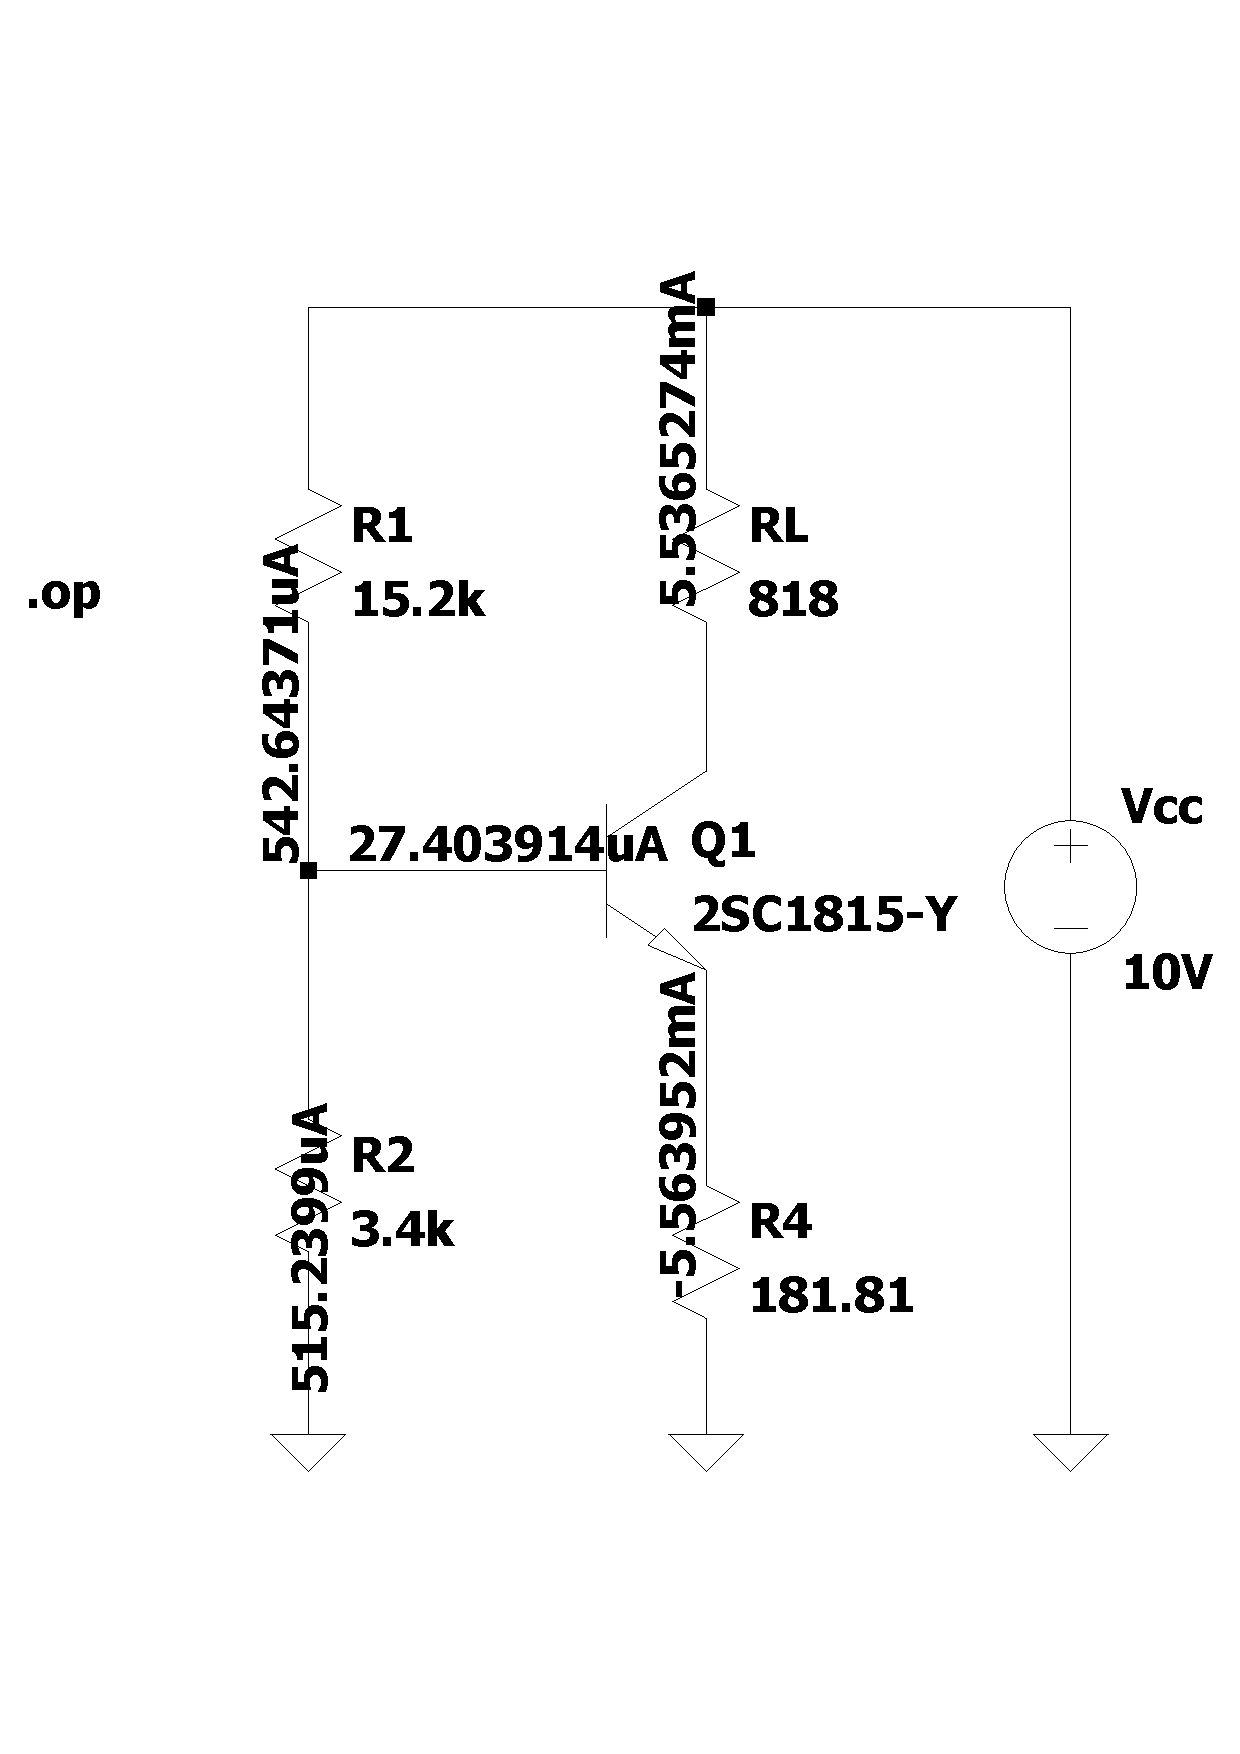
\includegraphics[width=0.4\linewidth]{img/44.pdf}
    \caption{電流帰還バイアス回路DC動作点解析}
    \end{center}
  \end{figure}
\end{description}
\section{エミッタ接地交流増幅回路の設計(交流を含めた話)}
電流帰還バイアス回路を用いたエミッタ接地交流増幅回路を設計する。この回路が、実際に使用されるエミッタ接地回路である。

\begin{description}
  \setlength{\parskip}{0cm} % 段落間
  \setlength{\itemsep}{0cm} % 項目間
  \item[ゴール] 電流帰還バイアス回路を用いたエミッタ接地交流増幅回路を設計する。
  \item[キーワード] 等価回路、結合キャパシタ$C_1、C_2、C_E$、電圧増幅度、遮断周波数、入力インピーダンス、四端子定数、$V_{BE}-I_E$特性
  \item[ストーリー] エミッタ接地回路の交流成分を考える → 交流等価回路にする → 入力インピーダンス、出力インピーダンスをなんか計算する → 低域遮断周波数、電圧増幅度、結合キャパシタの値を決める。ついでに利得とかも計算する。→ LTspiceで設計 → LTspiceで交流増幅特性(AC解析) → LTspiceで過渡解析 → 計算値と比較
\end{description}

\subsection{原理・計算}
図にエミッタ接地交流増幅回路を示す。ここでは、どのキャパシタが入力信号を遮断周波数に影響を与えるかを考える。
\begin{figure}[htbp]
  \begin{center}
  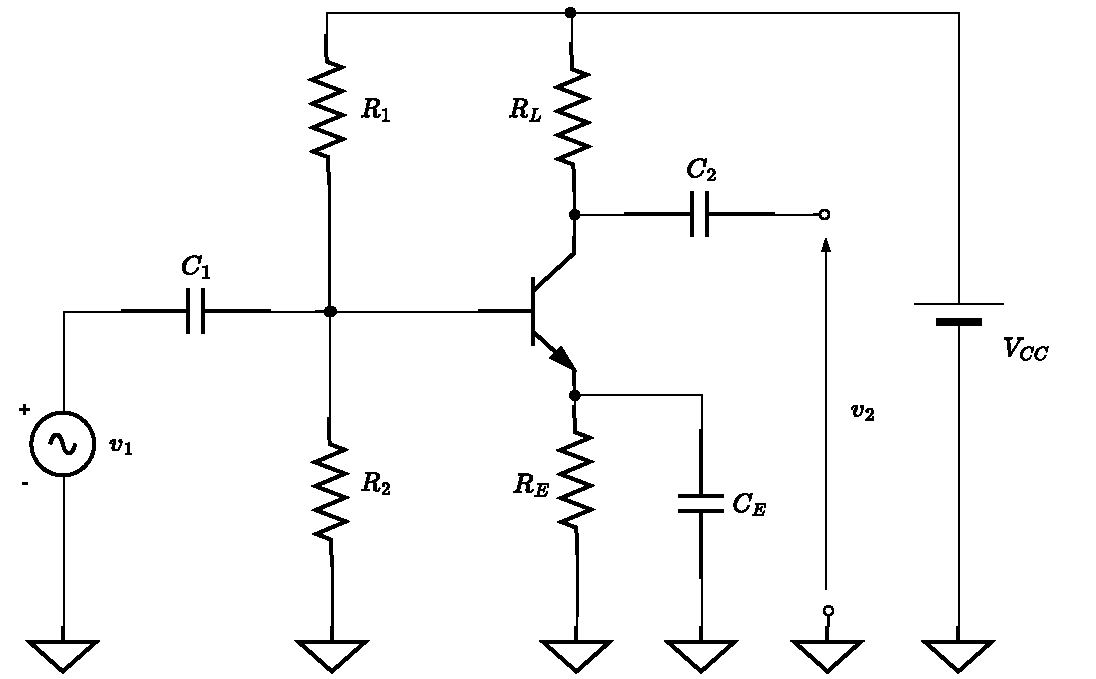
\includegraphics[width=0.68\linewidth]{img/45.pdf}
  \caption{エミッタ接地交流増幅回路}
  \end{center}
\end{figure}

$C_{E}$: バイパスキャパシタ\\
$C_{1}, C_{2}$: 結合キャパシタ(直流信号を遮断して交流信号だけを通過)

\subsubsection{等価回路}
エミッタ接地微小信号等価回路と微小信号の変化分を表す特性を図に示す。
微小信号とは、小さな振幅の交流信号のことである。
$r_e$ は、ベース - エミッタ間の pn 接合ダイオードを抵抗に置き換えたものである。
直流に対しては、この pn 接合はダイオードと考えられるが、ベースの入力信号が微小変化する場合には、$V_{BE}$ の変化に対してエミッタ電流 $I_E$ の変化が比例して変化するものと考えられる。
\begin{figure}[htb]
  \begin{center}
  \subfigure[エミッタ接地微小信号等価回路]{
  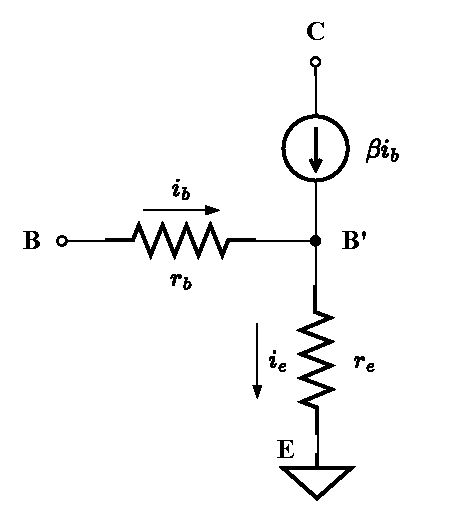
\includegraphics[width=.45\columnwidth]{img/46.pdf}
  }
  \subfigure[微小信号の変化分を表す特性($V_{BE}$-$I_E$特性の再喝)]{
  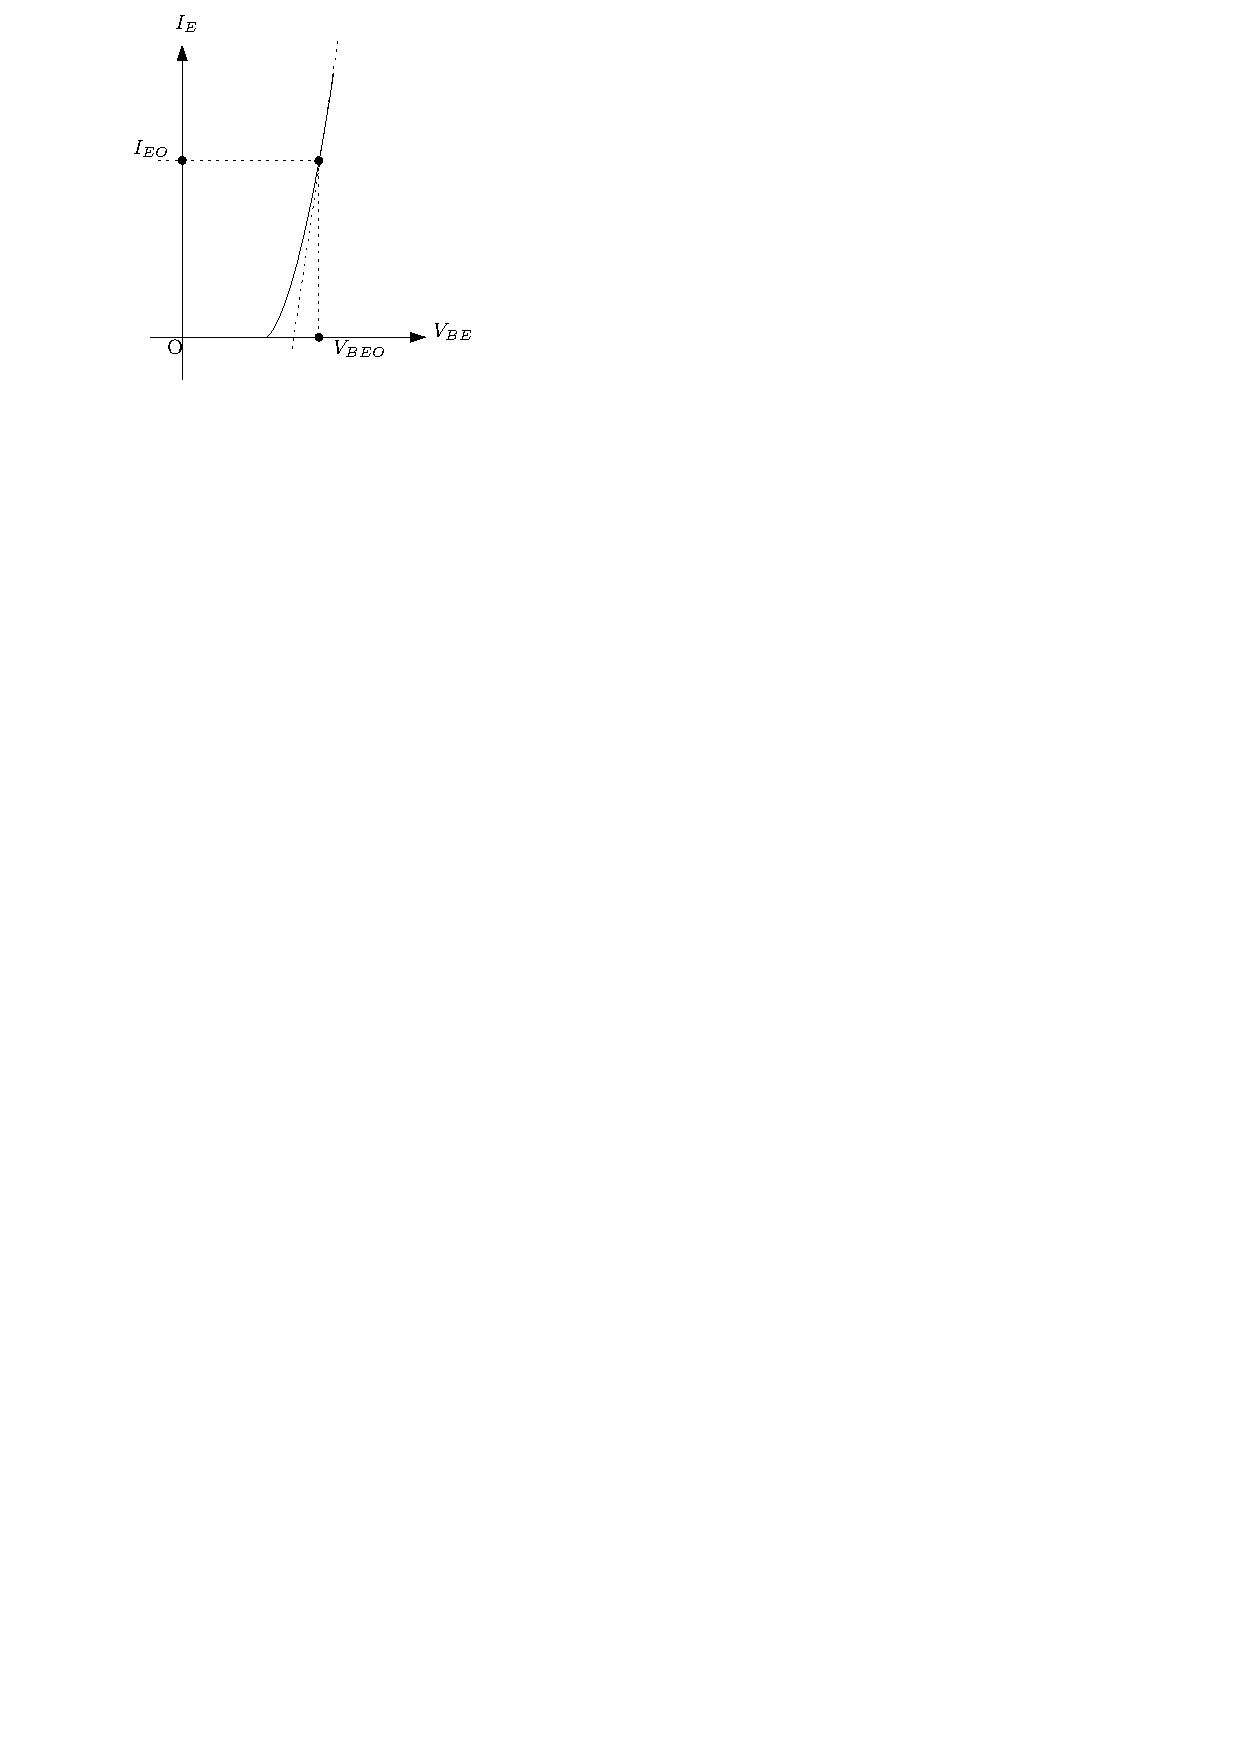
\includegraphics[width=.45\columnwidth]{img/47.pdf}
  }
  \caption{微小信号等価回路の原理}
  \end{center}
\end{figure}

$I_E \approx I_S \exp(\frac{q}{kT}V_{BE})$ を $V_{BE}$ で微分すると(これが、$I_E$-$V_{BE}$曲線の傾きとなる。)\\
$$\frac{1}{r_e} = \frac{dI_E}{dV_{BE}} \approx \frac{q}{kT}I_S\exp(\frac{q}{kT}V_{BE}) = \frac{q}{kT}I_E$$
$$r_e = \frac{kT}{q}\cdot\frac{1}{I_{EO}} \approx \frac{0.026}{I_{EO}}$$

\subsubsection{電圧増幅度の計算}
微小信号等価回路を利用して描いた交流等価回路を示す。
\begin{figure}[htbp]
  \begin{center}
  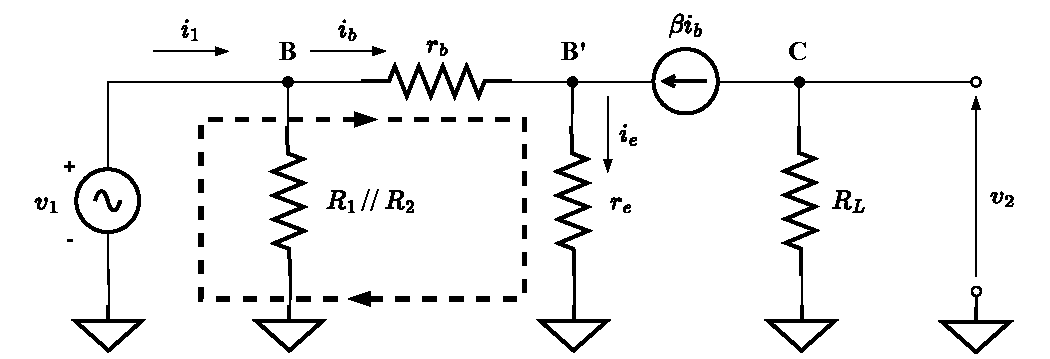
\includegraphics[width=0.8\linewidth]{img/48.pdf}
  \caption{エミッタ接地交流増幅回路の等価回路}
  \end{center}
\end{figure}

\begin{description}
  \item [入力インピーダンス]: $R_1//R_2$と$Z_i$が並列に接続されている。\\
  ($Z_i$は、ベース端子から見た入力インピーダンス)
  ここで、$Z_i = v_1/i_b$より、点線のループに沿ってキルヒホッフの法則を適用すると、
  $$v_1 = r_bi_b+r_ei_e\dots1$$
  B'点にキルヒホッフの電流則を適用すると、$i_e = (1+\beta)i_b\dots$2\\
  1、2より、$i_e$ を消去して、$v_1 = r_bi_b+r_e(1+\beta)i_b$\\
よってベースから見た入力インピーダンス $Z_i$ は、$Z_i = \frac{v_1}{i_b} = r_b+(1+\beta)r_e$\\
$Z_i$ を用いると、エミッタ接地回路の入力端子から見たインピーダンス $Z_{in}$ は、\\
$Z_{in} = R_1//R_2//Z_i$ となる。
  \item [電圧増幅度]: 負荷抵抗 $R_L$ には下から上に流れる電流 $\beta i_b$ が流れている。\\
  よって、出力電圧 $v_2$ は、逆の極性を持つため、\\
  $$v_2 = - R_L\beta i_b$$
  $$i_b = \frac{v_1}{r_b+(1+\beta)r_e}$$
  $$A_v = \frac{v_2}{v_1} = \frac{-\beta R_L}{r_b+(1+\beta)r_e} = \frac{-\beta R_L}{Z_i}$$
\end{description}

\subsubsection{$C_1$ による遮断周波数 $f_{C1}$}
  入力側の結合キャパシタ $C_1$を考慮した入力部の等価回路を図に示す。

  \begin{figure}[htbp]
    \begin{center}
    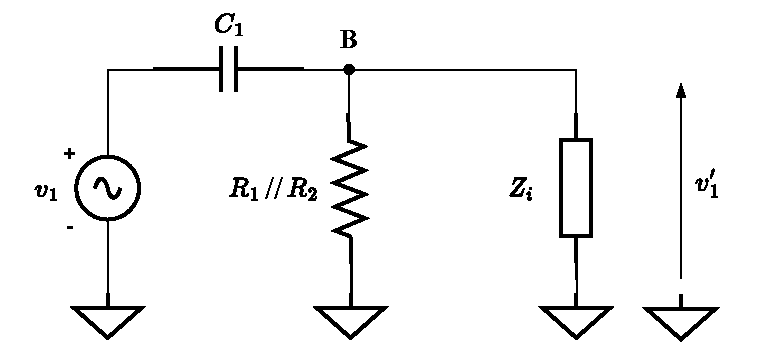
\includegraphics[width=0.8\linewidth]{img/49.pdf}
    \caption{$C_1$を考慮したエミッタ接地交流増幅回路の等価回路}
    \end{center}
  \end{figure}
  $v_1'$: ベースへの交流入力電圧 $v_1$: 元の入力信号として、\\
  電圧 $v_1$$v_1'$との比を求めると、
  $$\frac{v_1'}{v_1} = \frac{R_1//R_2//Z_i}{\frac{1}{j\omega C_1}+R_1//R_2//Z_i} = \frac{1}{1+\frac{1}{j\omega C_1(R_1//R_2//Z_i)}}$$
  $$Z_i = \frac{v_1}{i_b} = r_b+(1+\beta)r_e$$
  キャパシタ $C_1$ を入れた時の電圧増幅度 $A'_v = \frac{v_2}{v_1}$ は、$A_v = \frac{v_2}{v'_1}$ として、
  $$A'_v = \frac{v_2}{v_1} = \frac{v'_1}{v_1}\cdot\frac{v_2}{v'_1} = A_v\frac{v'_1}{v_1} = \frac{-\beta R_L}{Z_i} \cdot \frac{1}{1+\frac{1}{j\omega C_1(R_1//R_2//Z_i)}}$$
  $A'_v$ の絶対値、(振幅伝達関数)は、
  $$|A'_v| = \frac{\beta R_L}{Z_i} \times \frac{1}{\sqrt{1+(\frac{1}{\omega C_1(R_1//R_2//Z_i})^2}}$$となる。
  $\frac{\beta R_L}{Z_i}$は、全てのキャパシタを短絡して考えた $A_v$ の式と同じである。
  この増幅度から、$\frac{1}{\sqrt{2}}$ に低下する周波数(低域遮断周波数$f_{C1}$)は、
  $$\omega C_1(R_1//R_2//Z_i) = 1より、$$
  $$2\pi f_{C1}C_1(R_1 \verb|//| R_2 \verb|//| Z_i) = 1$$
  $$C_1 = \frac{1}{2\pi f_{C1} (R_1//R_2//Z_i)} = 1$$

\subsubsection{$C_2$による遮断周波数$f_{C2}$}
入力側の結合キャパシタ$C_2$を入れた入力部の等価回路を図に示す。
\begin{figure}[htbp]
  \begin{center}
  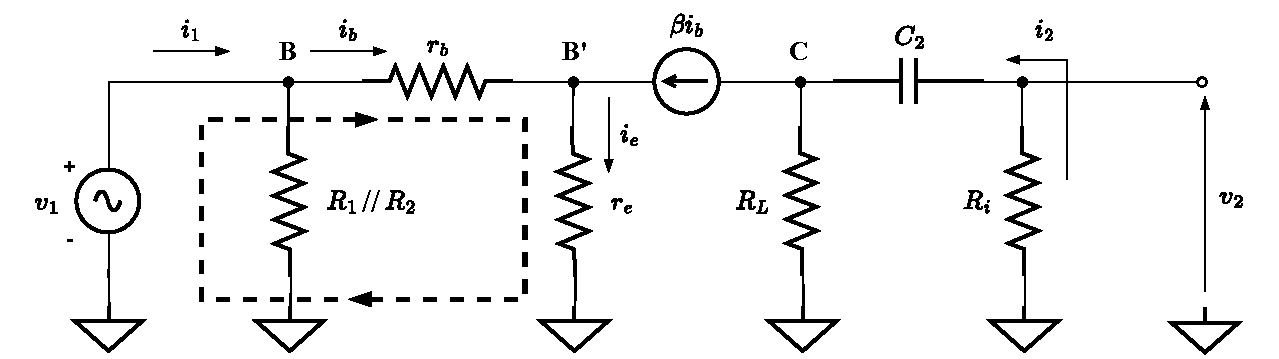
\includegraphics[width=0.8\linewidth]{img/50.pdf}
  \caption{$C_2$を考慮したエミッタ接地交流増幅回路の等価回路}
  \end{center}
\end{figure}
図の点線に沿ってキルヒホッフの電圧則を適用すると、
$$v_1 = r_bi_b+(1+\beta)r_ei_b$$
出力側に流れる電流$i_2$を電流源$\beta i_b$から求めると、出力側の回路は$R_L$と、直列の$C_2-R_i$が並列接続された形であるため、\\
$$i_2 = \beta i_b \times \frac{R_L}{R_L+(\frac{1}{j\omega C_2}+R_i)}$$ で求まる。また、出力側電圧$v_2$は、
$$v_2 = - i_2R_i$$
よって、電圧増幅度$A_v$は、
$$A_v = \frac{v_2}{v_1} = \frac{-i_2R_i}{r_bi_b+(1+\beta)r_ei_b} = \frac{\frac{-\beta R_LR_i}{R_L+(\frac{1}{j\omega C_2}+R_i)}}{r_b+(1+\beta)r_e}$$
$$= \frac{-\beta}{r_bi_b+(1+\beta)r_ei_b} \cdot \frac{R_LR_i}{R_L+(\frac{1}{j\omega C_2}+R_i)} = \frac{-\beta}{r_bi_b+(1+\beta)r_ei_b} \cdot \frac{\frac{R_LR_i}{R_L+R_i}}{1+\frac{1}{j\omega C_2(R_L+R_i)}}$$
$$= \frac{-\beta R'_L}{r_bi_b+(1+\beta)r_ei_b} \cdot \frac{1}{1+\frac{1}{j\omega C_2(R_L+R_i)}}$$
と求まる。($R'_L = R_L//R_i$)\\
$\frac{-\beta R'_L}{Z_i} \cdot \frac{1}{1+\frac{1}{j\omega C_2(R_L+R_i)}}$ と、$-\frac{\beta R_L}{Z_i}$ と見比べると、$C_2$ を短絡して考えられる 周蓮での増幅度に相当する。つまり、$R_L$ と次段の入力インピーダンス $R_i$ が並列接続された形で増幅度が決まる。
$$|A_v| = \frac{\beta R'_L}{Z_i} \cdot \frac{1}{\sqrt{1+(\frac{1}{(\omega C_2(R_L+R_i)})^2}}$$
$C_2$ を短絡して考えた場合の値 $\frac{\beta R'_L}{Z_i}$ に対して、増幅度が $1/sqrt{2}$ となる周波数(低域遮断周波数 $f_{C2}$)は、$\omega C_2(R_L+R_i) = 1$、$2\pi f_{C2} C_2(R_L+R_i) = 1$ より、\\
$$f_{C2} = \frac{1}{2\pi C_2(R_L+R_i)}$$

\subsubsection{$C_E$による遮断周波数 $f_{CE}$}
抵抗 $R_E$ に並列にバイパスキャパシタ$C_E$を入れた等価回路を図に示す。
\begin{figure}[htbp]
  \begin{center}
  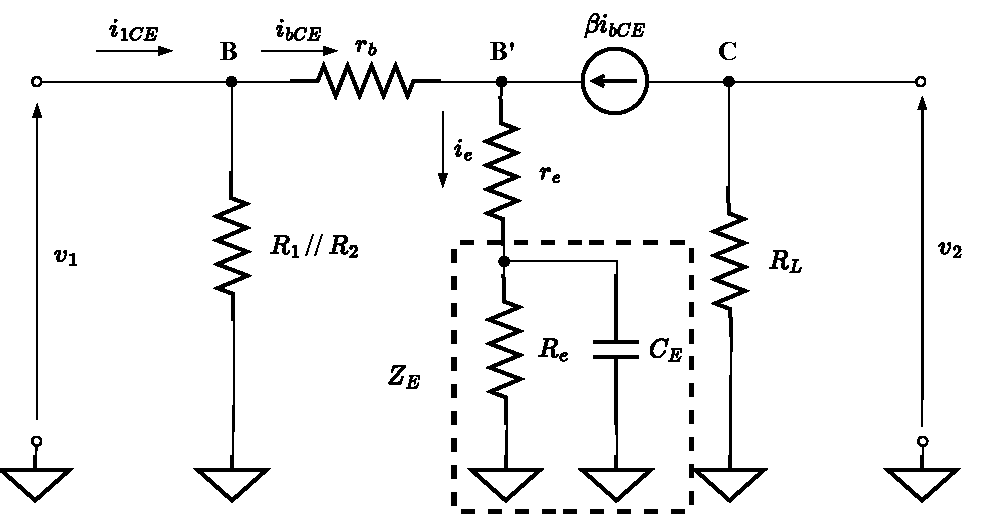
\includegraphics[width=0.8\linewidth]{img/51.pdf}
  \caption{$C_E$を考慮したエミッタ接地交流増幅回路の等価回路}
  \end{center}
\end{figure}

$C_E, R_E$ の並列インピーダンス $Z_E$は、$$Z_E = \frac{R_E \cdot \frac{1}{j\omega C_E}}{R_E+\frac{1}{j\omega C_E}} = \frac{R_E}{1+j\omega C_ER_E}\dots1$$
$C_E$ が短絡している場合、$Z_E = 0$ となる。$v_1 \rightarrow r_b \rightarrow r_e$のループにキルヒホッフの電圧則を適用した式 $v_1 = r_bi_{bCE}+r_e(1+\beta)i_{bCE}$ を用いて、
$Z_i = \frac{v_1}{i_{bCE}} = r_b+(1+\beta)r_e$ とある。
ベース端子B から見たトランジスタの入力インピーダンス\\

$r_b: 50 ～ 500 \Omega$ 程度 $\beta$: 100 ~ 500 程度 ダイオードの交流等価回路 $r_e$: 数10 $\Omega$ $(1+\beta)r_e >> r_b, \beta >> 1$ として、
$Z_i \approx (1+\beta)r_e \approx \beta r_e\dots2$となる。
電圧増幅度 $A_v = \frac{v_2}{v_1}$ について、$v_1 \rightarrow r_b \rightarrow r_e \rightarrow Z_E$ のループにキルヒホッフの電圧則を適用すると

$v_1 = r_b i_{bCE}+(r_e+Z_E)(1+\beta)i_{bCE}$
$= [r_b+(1+\beta)(r_e+Z_E)]i_{bCE} = [r_b+(1+\beta)r_e+(1+\beta)Z_E]i_{bCE}$
$= [Z_i+(1+\beta)Z_E]i_{bCE}$ となる。
$v_2 = -R_L\beta i_{bCE}$ ($v_2$ は、電流$\beta i_{bCE}$ が負荷抵抗 $R_L$ を下から上に流れる。)
$$A_v = \frac{v_2}{v_1} =\frac{-\beta R_L}{Z_i+(1+\beta)Z_E}\dots3$$
3を1,2に代入して、
$$A_v = \frac{-\beta R_L}{Z_i+(1+\beta)Z_E} \approx \frac{-\beta R_L}{Z_i+\beta \frac{R_E}{1+j\omega C_E R_E}}$$
$$= \frac{-\beta R_L(1+j\omega C_E R_E)}{Z_i(1+j\omega C_ER_E)+\beta R_E} = -\beta R_L \cdot \frac{1+j\omega C_E R_E}{Z_i+\beta R_E+j\omega C_ER_EZ_i} \approx -\beta R_L \cdot \frac{1+j\omega C_E R_E}{\beta r_e+\beta R_E + j\omega C_E R_E Z_i}$$
$$= -\beta R_L R_E \cdot \frac{1+j\omega C_ER_E}{\beta(r_e+R_E)+j\omega C_E R_E Z_i} \approx -\beta R_L \cdot \frac{1+j\omega C_E R_E}{\beta R_E + j\omega C_E R_E Z_i}$$
$$= -\frac{\beta R_L}{R_E} \cdot \frac{1+j\omega C_E R_E}{\beta + j\omega C_E Z_i} = -\frac{R_L}{R_E} \cdot \frac{1+j\omega C_E R_E}{1+j\omega C_E Z_i/\beta}\dots4$$
2より、$$A_v \approx -\frac{R_L}{R_E}\cdot\frac{1+j\omega C_ER_E}{1+j\omega C_EZ_i/\beta} \approx -\frac{R_L}{R_E}\cdot \frac{1+j\omega C_E R_E}{1+j\omega C_E r_e}$$

$f \to \infty, \omega \to \infty$ の場合、\\
$\left.A_v\right|_{\omega \to 0} \approx -\frac{R_L}{R_E}$ と一定値(低域の電圧増幅度) になり、\\
$\left.A_v\right|_{\omega \to \infty} \approx -\frac{R_L}{r_e} \leftarrow$ ロピタルの定理\\
と、一定値(中域での電圧増幅度)となる。

$-\frac{R_L}{R_E} \cdot \frac{1+j\omega C_E R_E}{1+j\omega C_E r_e}$ の分母分子に関係する特徴的な周波数について

$$f_{CE1} = \frac{1}{2\pi C_E Z_i/\beta} \approx \frac{1}{2\pi C_E r_e}$$
$$f_{CE2} = \frac{1}{2\pi C_E R_E}$$
$$A_v \approx -\frac{R_L}{R_E} \cdot \frac{1+j(f/f_{CE2})}{1+j(f/f_{CE1})}$$

$$A_v \approx -\frac{R_L}{R_E} \cdot \frac{1+j(f/f_{CE2})}{1+j(f/f_{CE1})}$$
$$|A_v| \approx \frac{R_L}{R_E} \cdot \sqrt{\frac{1+(f/f_{CE2})^2}{1+(f/f_{CE1})^2}}$$
この式は、低周波数側から周波数を増加させるとき、$f_{CE2}, f_{CE1}$ で2回折れ曲がる形の関数である。

$f_{CE2}$ は、$C_E R_E$ で決まる周波数
低周波数 → 高周波数に増加するときに増幅度が上りはじめる周波数

$f_{CE1}$ は、時定数 $C_E r_e$ で決まる周波数で、高周波 → 低周波数に減少するときに
増幅度が下がりはじめる周波数である。したがって、バイパスキャパシタ $C_E$ を含む図の等価回路では、低域遮断周波数は、$f_{CE1}$ となる。

\subsubsection{低域遮断周波数のまとめ}
入力側キャパシタ $C_1$: $f_{C1} = \frac{1}{2\pi C_1(R_1//R_2//Z_i)}$\\
出力側キャパシタ $C_2$: $f_{C2} = \frac{1}{2\pi C_2(R_L+R_i)}$\\
バイパスキャパシタ $C_E$: $f_{CE1} = \frac{1}{2\pi C_E Z_i/\beta} \approx \frac{1}{2\pi C_E r_e}$\\

$R_1, R_2, R_L, R_i, Z_i$ が、k$\Omega$ オーダに対し、$r_e \approx \frac{Z_i}{\beta}$ は、\\
1 ～ 10 $\Omega$ オーダ各キャパシタの静電容量を同じにすると、$C_E$ による周波数 $f_{CE1}$ が最も大きな値となる。つまり、低域遮断周波数は、トランジスタの交流増幅率の低下、ベース- コレクタ間容量によるベース端子への逆位相信号入力(負帰還)、回路を組み立てる配線の分布容量など複数の要因がからみ合っており、高域遮断周波数の設計には、より高度な回路に関する知見が必要である。

\subsubsection{諸量計算$r_e$、$A_v$、低域遮断周波数}
$r_e, A_v(電圧増幅度), 低域遮断周波数 f_{CE1}, f_{C1}, f_{C2}$\\
条件1 $C_1, C_2$は、$100 \mu$F を使う\\
\begin{enumerate}
  \setlength{\parskip}{0cm} % 段落間
  \setlength{\itemsep}{0cm} % 項目間
  \item $r_e \approx \frac{kT}{q} \cdot \frac{1}{I_{EQ}}$
  $r_e \approx \frac{0.026}{I_{EO}} (I_{EO} \approx I_{CO}) (\frac{kT}{q} は定数)$
  \item $A_v = \frac{v_2}{v_1} = -\frac{\beta R_L}{Z_i} = -\frac{R_L}{Z_i/\beta} \approx -\frac{R_L}{r_e} = \frac{506}{3.3} \approx -153$
\end{enumerate}

条件2: 低域遮断周波数$f_{CE1} = 20$ Hz として設計)
$$f_{CE1} \approx \frac{1}{2\pi C_E r_e} \Rightarrow C_E \approx \frac{1}{2\pi f_{CE1}r_e}$$


\subsection{エミッタ接地交流増幅回路の設計手順}
\begin{enumerate}
  \setlength{\parskip}{0cm}
  \setlength{\itemsep}{0cm}
  \item $r_e \approx \frac{0.026}{I_{EO}} \approx \frac{0.026}{I_{CO}} = \frac{26\times10^{-3}}{5.5 \times 10^{-3}} \approx 4.7272 [\Omega]$
  \item $A_v = \frac{v_2}{v_1} = -\frac{\beta R_L}{Z_i} = -\frac{R_L}{Z_i/\beta} \approx -\frac{818.18}{4.72} = -173.3432...$
  \item $C_E$: 低域遮断周波数を 20 Hz として設定(可聴周波数の下限)\\
  $f_{CE1} \approx \frac{1}{2\pi C_Er_e} \Rightarrow C_E \approx \frac{1}{2\pi f_{CE1} r_e} \approx \frac{1}{2\pi \times 20 \times 4.72} = 1.68596 \times 10^{-3} = 1686 \mu\textrm{F}$
\end{enumerate}
$C_1, C_2は、100 \mu\textrm{F} より、次段の入力インピーダンスを R_i = 1\textrm{k}\Omega と仮定$

$f_{C1} = \frac{1}{2\pi C_1(R_1//R_2//Z_i)} \approx \frac{10^4}{2\pi \times (15.2\times10^3//3.4\times10^3//10^3)} \approx \frac{10^4}{2\pi \times 735.344} \approx 2.1643\textrm{Hz}$\\
$f_{C2} = \frac{1}{2\pi C_2(R_L+R_i)} \approx \frac{1}{2\pi \times 10^{-4} \times 1.818 \times 10^3} = 0.8754[\textrm{Hz}]$\\
$f_{C1}, f_{C2}$は、20 Hz と比べてかなり小さい。


\subsection{LTSpiceで演習}
バイアス設定確認 → 動作点解析 → 交流増幅特性解析の順に行う。
$C_2$ の出力側に次段の入力インピーダンス $R_i = 1$k$\Omega$ を接続することで、中域の増幅度が変化する。


$電圧増幅度(中域) |A_v| = \frac{\beta R'_L}{Z_i} = \frac{R'_L}{Z_i/\beta} \approx \frac{R'_L}{r_e}
(R'_L = R_L//R_i = \frac{R_LR_i}{R_L+R_i})$

$電圧利得 20 \log (R'_L/r_e)$

\subsubsection{過渡解析(中域の増幅度に関して)}
\begin{enumerate}
  \setlength{\parskip}{0cm}
  \setlength{\itemsep}{0cm}  
  \item $v_1 = 10$mV (振幅), 1 kHz
  \item $R_i$ の次段の入力抵抗を1k$\Omega$
  \item $R'_L = R_L \verb|//| R_i$ より、$R_i$ は、中域の増幅度に影響を与える。
\end{enumerate}
中域増幅度 $|A_v| = \frac{\beta R'_L}{Z_i} = \frac{R'_L}{Z_i/\beta} \approx \frac{R'_L}{r_e}$より、\\
$$R'_L = R_L \verb|//| R_i = 818.18 \verb|//| 10^{3} = 449.999... \fallingdotseq 450[\Omega]$$
$$電圧増幅率 |A_v| \approx \frac{R'_L}{r_e} = \frac{450}{4.7272...} = 95.1937... \fallingdotseq 95$$
$$電圧利得 20\log(\frac{R'_L}{r_e}) = 20\log(\frac{450}{4.7272...}) = 39.572... \fallingdotseq 39.6\textrm{dB}$$

\begin{description}
  \item[課題11] 入力信号 $v_1 =$ 20 mVp-p 1kHz として以下の回路を設計し、下図のような過渡特性を取得して下さい。 
  \begin{figure}[htbp]
    \begin{center}
    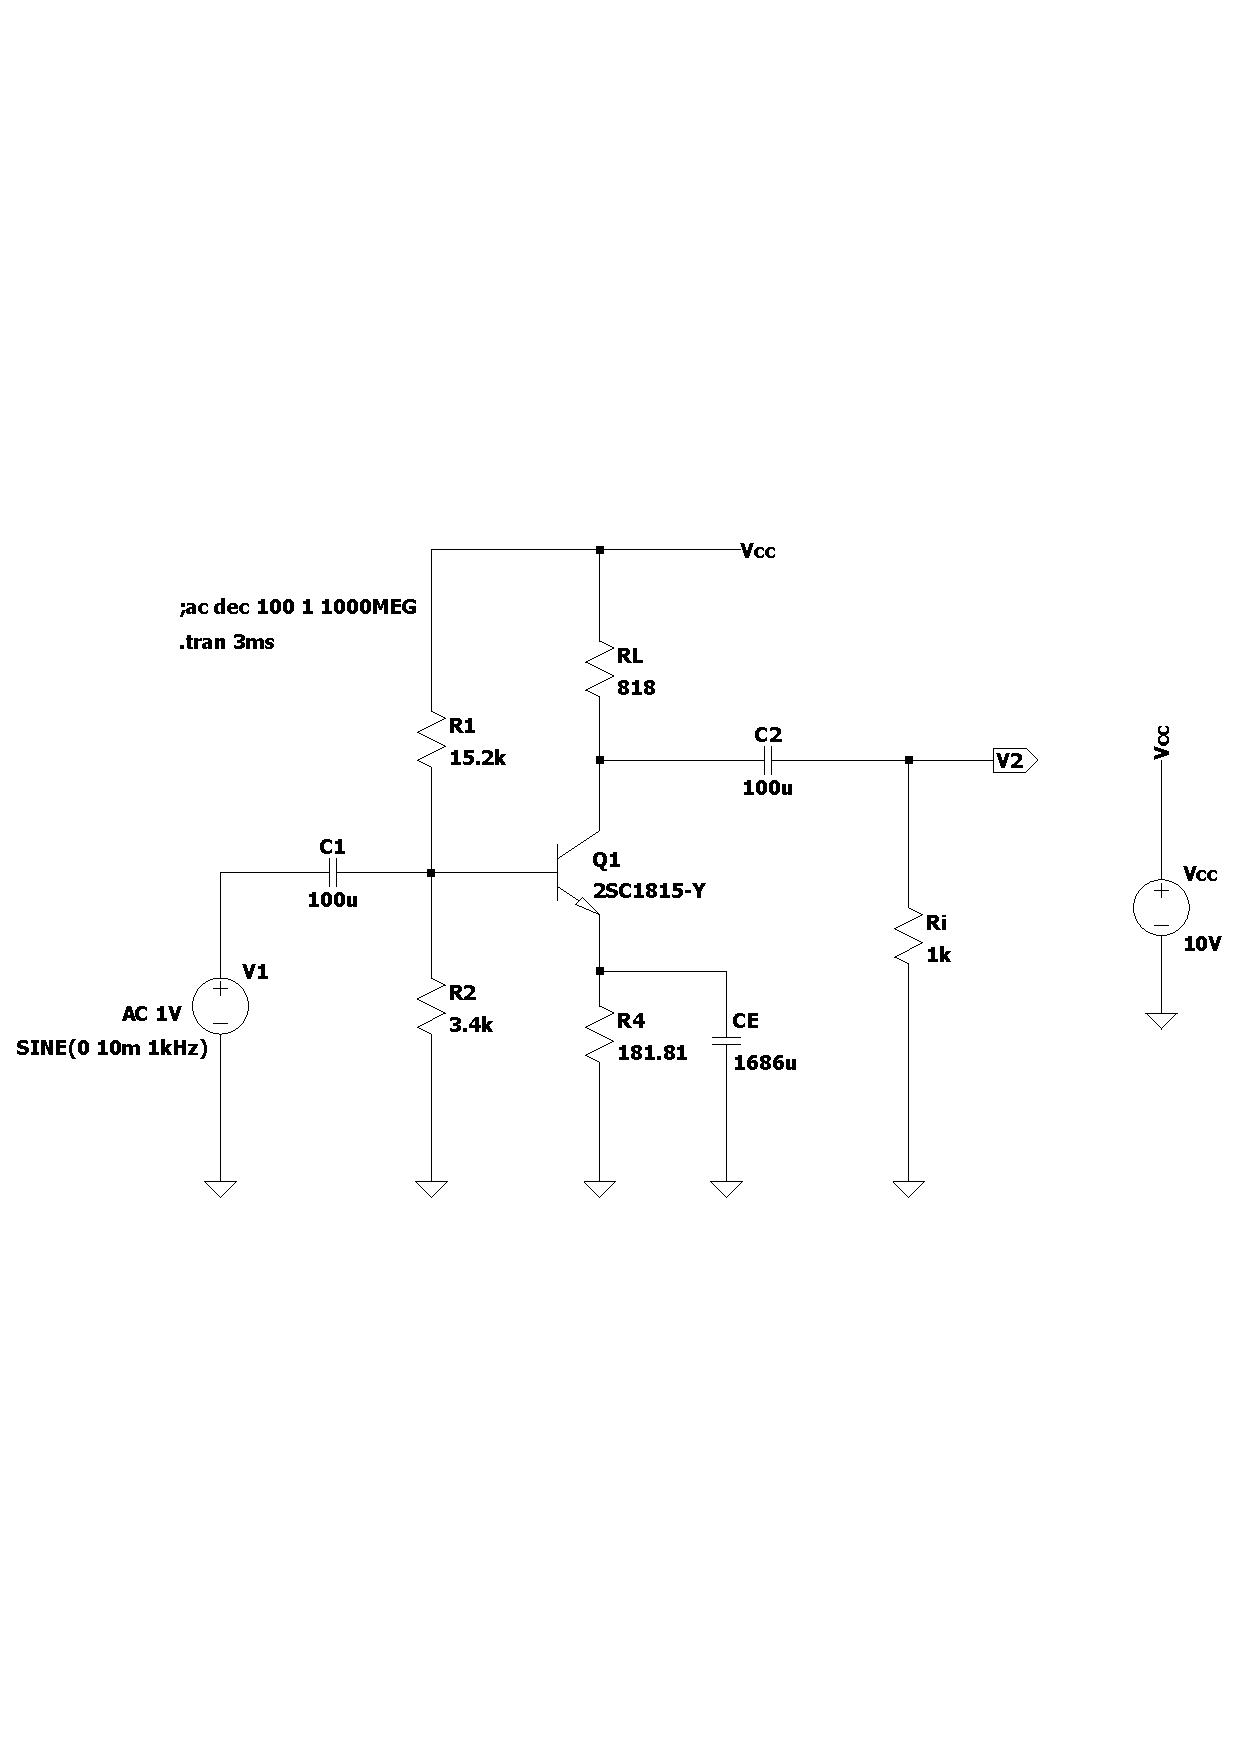
\includegraphics[width=\linewidth]{img/52.pdf}
    \caption{エミッタ接地交流増幅回路}
    \end{center}
  \end{figure}
  \begin{figure}[htbp]
    \begin{center}
    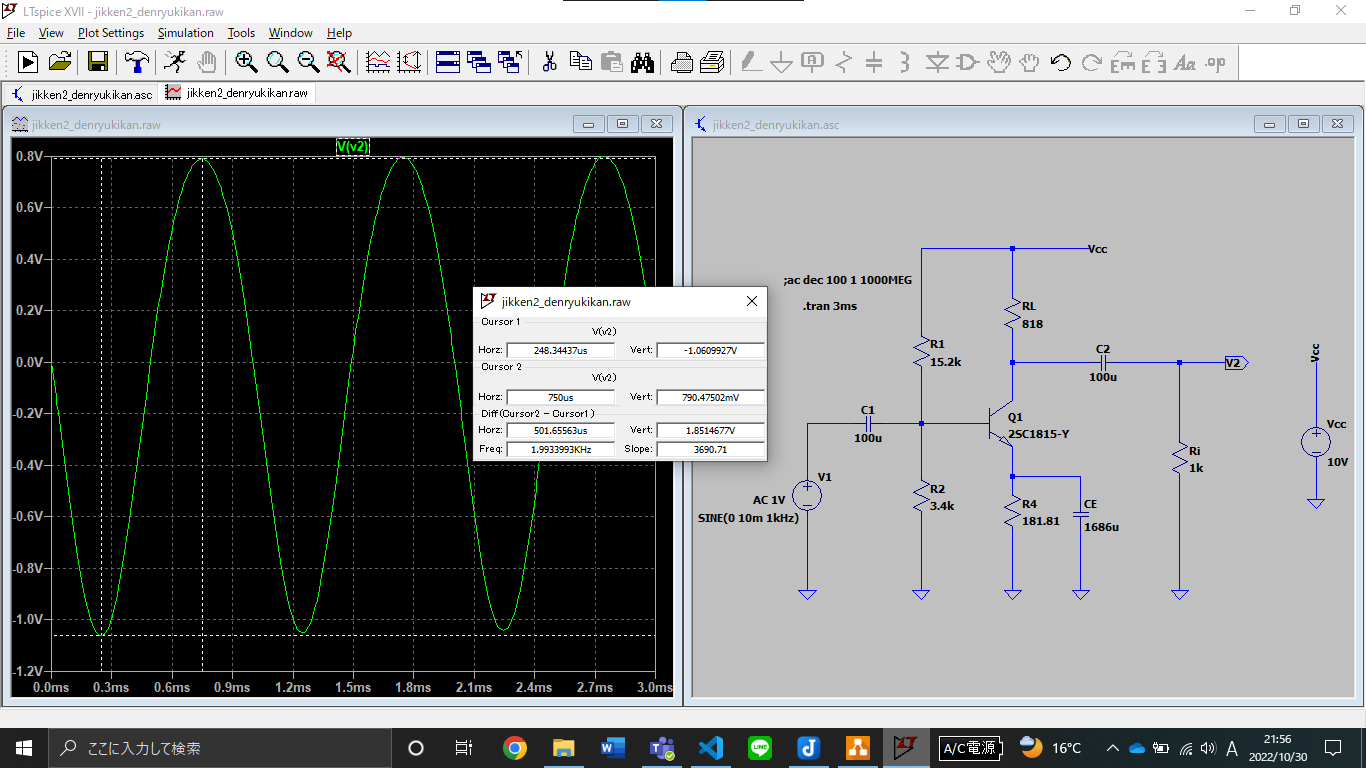
\includegraphics[width=\linewidth]{img/53.png}
    \caption{過渡特性}
    \end{center}
  \end{figure}
\end{description}

\subsubsection{AC解析}
\begin{description}
  \item[課題12] 手順に沿って下図のようなAC解析を行って下さい。\\
「Edit Simulation Command.」→ 「AC解析」→ 「Stop frequency」を"100MEG"に設定 → .ac ディレクティブを回路図に張り付けて「Run」を実行する。
電圧プローブを$v_2$ に設定する。

\begin{figure}[htbp]
  \begin{center}
  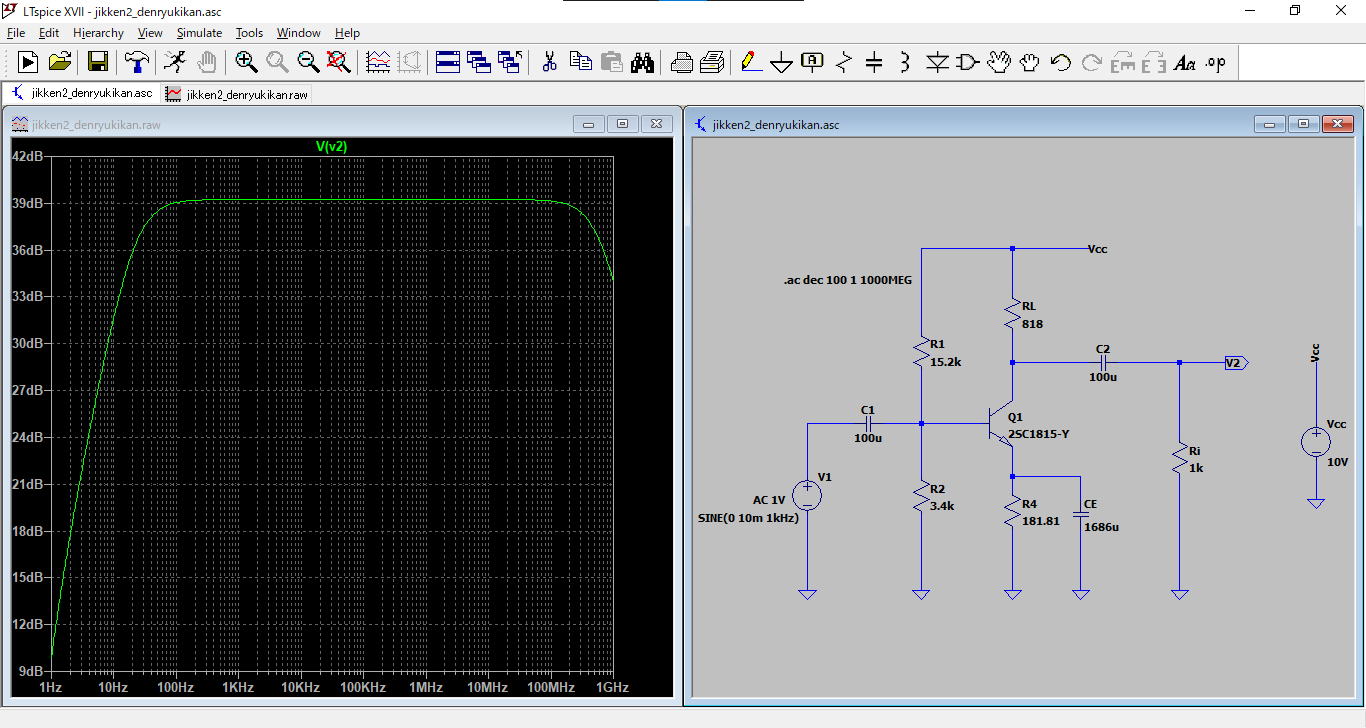
\includegraphics[width=.7\linewidth]{img/54.png}
  \caption{AC解析}
  \end{center}
\end{figure}

  \item [課題13] 設定した低域遮断周波数、電圧増幅率、電圧利得を、グラフから読み取り、理論値と実測値で比較してください。\\
  低域遮断周波数: 電圧利得が 3dB 降下する周波数\\
  電圧増幅率: 過渡解析において、$v_2$ のp-p 値を求め、$v_2/v_1$ の値を求める。\\
  電圧利得: $20\log|A_v|$ の値をAC解析の中域利得と比較する。
\begin{figure}[htbp]
  \begin{center}
  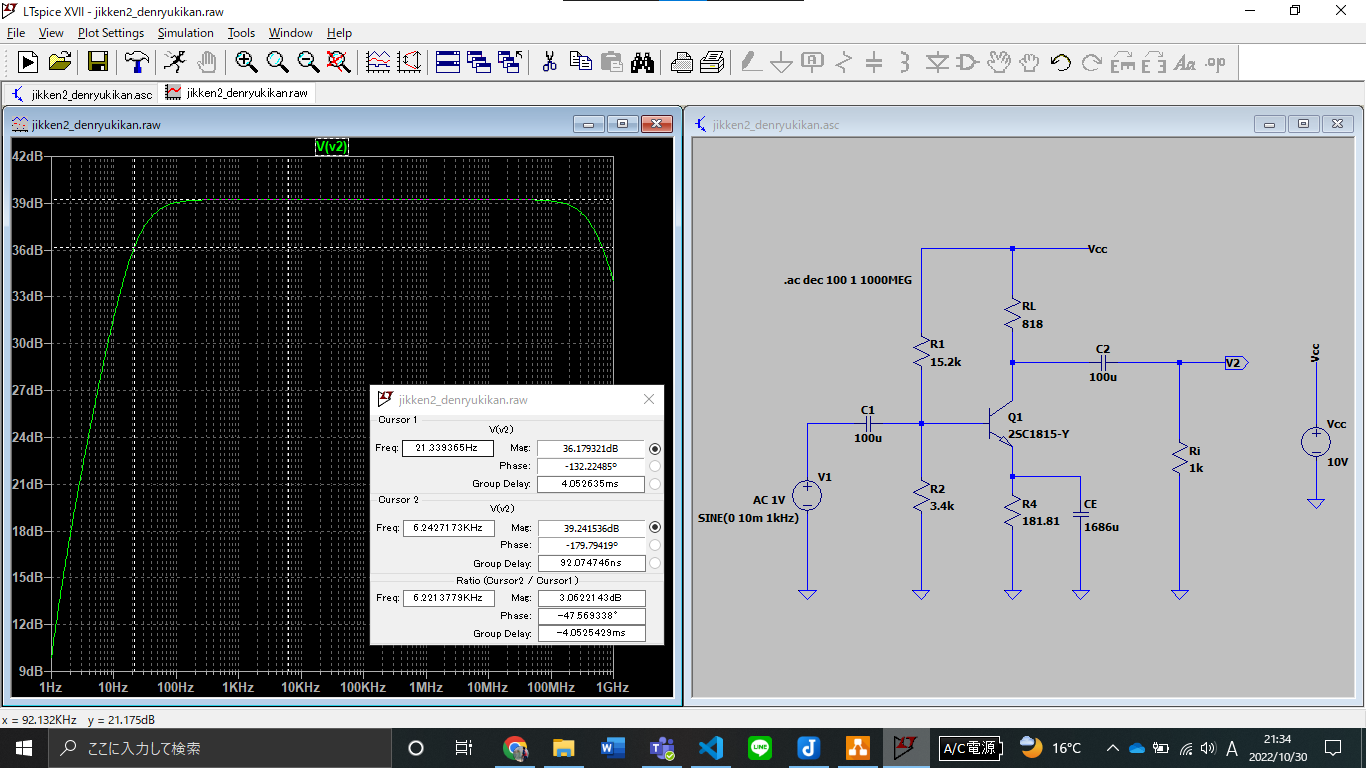
\includegraphics[width=.7\linewidth]{img/55.png}
  \caption{AC特性(3dB降下をカーソルで取得)}
  \end{center}
\end{figure}
\end{description}


\pagestyle{plain}
\bibliographystyle{jplain}
\addcontentsline{toc}{section}{参考文献}
\begin{thebibliography}{3}
\bibitem{1}
鹿間信介（2022）, 
LTspiceで独習できる! はじめての電子回路設計. 
講談社, 2022.

\bibitem{2}
「エミッタ接地回路の『特徴』や『原理』について」\\{\it https://detail-infomation.com/amplifier-common-emitter-circuit/}\\
(最終アクセス　2022年11月1日)


\bibitem{3}
「トランジスタ(2SC1815)によるエミッタ接地回路【4】：電圧増幅回路の設計とLTSpiceによる詳細なシミュレーション｜たぬしの空想半径」, {\it https://tanukitanushi.com/rikei/circuit/emit4/}\\
(最終アクセス　2022年11月1日)
\end{thebibliography}

\end{document}